% ------------------------------------------------------------------------
%% abtex2-modelo-trabalho-academico.tex, v-1.7.1 laurocesar
%% Copyright 2012-2013 by abnTeX2 group at http://abntex2.googlecode.com/ 
% ------------------------------------------------------------------------

\documentclass[
	% -- opções da classe memoir --
	12pt,				% tamanho da fonte
	openright,			% capítulos começam em pág ímpar (insere página vazia caso preciso)
	oneside,			% para impressão em verso e anverso. Oposto a oneside
	a4paper,			% tamanho do papel. 
	% -- opções da classe abntex2 --
	chapter=TITLE,		% títulos de capítulos convertidos em letras maiúsculas
	section=TITLE,		% títulos de seções convertidos em letras maiúsculas
	%subsection=TITLE,	% títulos de subseções convertidos em letras maiúsculas
	%subsubsection=TITLE,% títulos de subsubseções convertidos em letras maiúsculas
	% -- opções do pacote babel --
	french,				% idioma adicional para hifenização
	spanish,			% idioma adicional para hifenização
	english,
	brazil,
	]{abntex2/abntex2}
	\renewcommand{\baselinestretch}{1.5} %para customizar o espaço entre as linhas do texto


% -----------------------------------------------------------
% PACOTES
% -----------------------------------------------------------
\usepackage{abntex2/abntex2-cin-ufpe}
\usepackage{pdfpages}           %para incluir pdf como páginas
\usepackage{float}
\usepackage{cmap}				% Mapear caracteres especiais no PDF
\usepackage{lmodern}			% Usa a fonte Latin Modern			
\usepackage[T1]{fontenc}		% Selecao de codigos de fonte.
\usepackage[utf8]{inputenc}		% Codificacao do documento (conversão automática dos acentos)
\usepackage{lastpage}			% Usado pela Ficha catalográfica
\usepackage{indentfirst}		% Indenta o primeiro parágrafo de cada seção.
%\usepackage{color}				% Controle das cores
\usepackage{graphicx}			% Inclusão de gráficos
\usepackage{lipsum}				% para geração de dummy text
\usepackage[versalete,alf,abnt-and-type=e,abnt-etal-list=0,abnt-etal-cite=3]{abntex2/abntex2cite} 
\usepackage{multirow}
\usepackage[section]{placeins}
\usepackage{lscape} 
\usepackage{rotating}           %rotates the figures, page
\usepackage{tikz}
\usepackage[section]{placeins}
\usepackage{setspace} 
\usepackage{inconsolata}
\usepackage{listings}
\usepackage{adjustbox}          % ajustar tabela ao tamanho da pagina
\usepackage{comandos}


% -----------------------------------------------------------
% CONFIGURAÇÃO DO DOCUMENTO
% -----------------------------------------------------------
% \usepackage[noframe]{showframe}
% \usepackage{showframe}

%\overfullrule=4mm %para identificar onde existem os alertas de linhas grandes mal formatada pelo LaTex, basta comentar para não aparecer a barra lateral preta na linha em questão.

\renewcommand*\arraystretch{1.2} %para customizar o espaço entre as linhas das tabelas



% -----------------------------------------------------------
% ABREVIATURAS E SIGLAS
% -----------------------------------------------------------
% \usepackage[noredefwarn,acronym]{glossaries} %GLOSSÁRIO
\usepackage[acronym,nonumberlist,nogroupskip,noredefwarn]{glossaries}
% \usepackage{glossary-superragged}

\newcolumntype{L}[1]{>{\raggedright\let\newline\\\arraybackslash\hspace{0pt}}m{#1}}
\newcolumntype{C}[1]{>{\centering\let\newline\\\arraybackslash\hspace{0pt}}m{#1}}
\newcolumntype{R}[1]{>{\raggedleft\let\newline\\\arraybackslash\hspace{0pt}}m{#1}}

\newglossarystyle{modsuper}{%
  %\glossarystyle{super}%
  \setglossarystyle{super}%
  \renewcommand{\glsgroupskip}{}
  
  % put the glossary in a longtable environment:
 \renewenvironment{theglossary}%
  {
    \begin{longtable}
        {L{0.2\textwidth}L{0.8\textwidth}}}%
    {\end{longtable}
  }%
}



% ----------------------------------------------------------
% CORES
% ----------------------------------------------------------
\definecolor{blue}{RGB}{41,5,195}
\definecolor{gray}{rgb}{.4,.4,.4}
\definecolor{gray}{rgb}{.4,.4,.4}
\definecolor{pblue}{rgb}{0.13,0.13,1}
\definecolor{pgreen}{rgb}{0,0.5,0}
\definecolor{pred}{rgb}{0.9,0,0}
\definecolor{pgrey}{rgb}{0.46,0.45,0.48}
\definecolor{lightgray}{rgb}{0.95, 0.95, 0.96}
\definecolor{whitesmoke}{rgb}{0.96, 0.96, 0.96}
\definecolor{javared}{rgb}{0.6,0,0} % for strings
\definecolor{javagreen}{rgb}{0.25,0.5,0.35} % comments
\definecolor{javapurple}{rgb}{0.5,0,0.35} % keywords
\definecolor{javadocblue}{rgb}{0.25,0.35,0.75} % javadoc
\definecolor{gray}{rgb}{0.5, 0.5, 0.5}
%\definecolor{lightgray}{gray}{0.9}


% ----------------------------------------------------------
% PERSONALIZAÇÃO DO USUÁRIO
% ----------------------------------------------------------
% ----------------------------------------------------------
% DADOS DO TRABALHO - CAPA e FOLHA DE ROSTO
% Configure os dados do trabalho aqui
% ----------------------------------------------------------
\titulo{Uma Abordagem Linguística para o Reconhecimento de Línguas de Sinais}
\autor{CLEISON CORREIA DE AMORIM}
\local{Recife}
\data{2022}
\areaconcentracao{\textbf{Área de Concentração}: Inteligência Computacional}
\orientador{\textbf{Orientador}: Cleber Zanchettin}
%\coorientador{\textbf{Coorientador (a)}: Texto Texto Texto}

\instituicao{UNIVERSIDADE FEDERAL DE PERNAMBUCO \\ CENTRO DE INFORMÁTICA \\ PROGRAMA DE PÓS-GRADUAÇÃO EM CIÊNCIA DA COMPUTAÇÃO}
\departamento{Centro de Informática}
\programa{Pós-graduação em Ciência da Computação}
\emailprograma{contato@cin.ufpe.br}
\siteprograma{http://www.cin.ufpe.br}

\tipotrabalho{Dissertação de Mestrado}

\preambulo{Trabalho apresentado ao Programa de Pós-Graduação em Ciência da Computação do Centro de Informática da Universidade Federal de Pernambuco, como requisito para obtenção do grau de Mestre em Ciência da Computação.}

% \preambuloatadefesa{Dissertação apresentada ao Programa de Pós-Graduação em Ciência da Computação da Universidade Federal de Pernambuco, como requisito para a obtenção do título de Mestre em Ciência da Computação, na data de ?? de Junho de 2022.}
% % TODO: ajustar data

%\input{userlists}



% ----------------------------------------------------------
% COMPILA O ÍNDICE
% ----------------------------------------------------------
\makeindex
% ---


% ----------------------------------------------------------
% ACRONIMOS
% ----------------------------------------------------------
% Lista de acrônimos:
\newacronym{oms}{OMS}{Organização Mundial da Saúde}
\newacronym{cfm}{CFM}{Conselho Federal de Medicina}
\newacronym{ibge}{IBGE}{Instituto Brasileiro de Geografia e Estatística}
\newacronym{ines}{INES}{Instituto Nacional de Educação de Surdos}
\newacronym{slr}{RLS}{Reconhecimento de Língua de Sinais}
\newacronym{ia}{IA}{Inteligência Artificial}
\newacronym{nlp}{PLN}{Processamento de Linguagem Natural}
\newacronym{mt}{TA}{Tradução Automática}
\newacronym{mhi}{MHI}{\textit{Motion History Image} (Imagem do Histórico de Movimento)}
\newacronym{mei}{MEI}{\textit{Motion Energy Image} (Imagem de Energia de Movimento)}
\newacronym{asllvd}{ASLLVD}{\textit{American Sign Language Lexicon Video Dataset}}
\newacronym{asllrp}{ASLLRP}{\textit{American Sign Language Linguistic Research Project}}
\newacronym{lstm}{LSTM}{\textit{Long Short-Term Memory}}
\newacronym{gru}{GRU}{\textit{Gated Recurrent Unit}}
\newacronym{rnn}{RNN}{\textit{Recurrent Neural Network} (Rede Neural Recorrente)}
\newacronym{cnn}{CNN}{\textit{Convolutional Neural Network} (Rede Neural Convolucional)}
\newacronym{ipa}{IPA}{\textit{International Phonetic Alphabet} (Alfabeto Fonético Internacional)}
\newacronym{sgd}{SGD}{\textit{Stochastic Gradient Descent
} (Gradiente Estocástico Descendente)}
\newacronym{pca}{PCA}{\textit{Principal Component Analysis
} (Análise de Componente Principal)}
\newacronym{hof}{HOF}{\textit{Histogram of Optical Flow
} (Histograma de Fluxo Óptico)}
\newacronym{hmm}{HMM}{\textit{Hidden Markov Model} (Modelos Ocultos de Markov)}
\newacronym{crf}{CRF}{\textit{Conditional Random Fields} 
(Campos Aleatórios Condicionais)}
\newacronym{cv}{VC}{Visão Computacional}
\newacronym{dl}{AP}{Aprendizagem Profunda}
\newacronym{ml}{AM}{Aprendizagem de Máquina}

% Línguas de sinais
\newacronym{asl}{ASL}{\textit{American Sign Language} (Língua de Sinais Americana)}
\newacronym{csl}{CSL}{\textit{Chinese Sign Language} (Língua de Sinais Chinesa)}
\newacronym{dgs}{DGS}{\textit{Deutsche Gebärdensprache} (Língua de Sinais Alemã)}
\newacronym{bsl}{BSL}{\textit{British Sign Language} (Língua de Sinais Britânica)}
\newacronym{arsl}{ArSL}{\textit{Arabic Sign Language} (Língua de Sinais Britânica)}
\newacronym{jsl}{JSL}{\textit{Japanese Sign Language} (Língua de Sinais Japonesa)}
\newacronym{isl}{ISL}{\textit{Indian Sign Language} (Língua de Sinais Indiana)}
\newacronym{gsl}{GSL}{\textit{Greek Sign Language} (Língua de Sinais Grega)}
\newacronym{tid}{TID}{\textit{Türk İşaret Dili} (Língua de Sinais Turca)}
\newacronym{ngt}{NGT}{\textit{Nederlandse Gebarentaal} (Língua de Sinais Holandesa)}
\newacronym{vgt}{VGT}{\textit{Vlaamse Gebarentaal} (Língua de Sinais Flamenga)}
\newacronym{lis}{LIS}{\textit{Lingua dei Segni Italiana} (Língua de Sinais Italiana)}
\newacronym{auslan}{AUSLAN}{\textit{Australian Sign Language} (Língua de Sinais Austrália)}
\newacronym{lsa}{LSA}{\textit{Lengua de Señas Argentina} (Língua de Sinais Argentina)}
\newacronym{tsl}{TSL}{\textit{Taiwan Sign Language} (Língua de Sinais de Taiwan)}
\newacronym{pjm}{PJM}{\textit{Polski Język Migowy} (Língua de Sinais Polonesa)}
\newacronym{libras}{Libras}{Língua Brasileira de Sinais}
\newacronym{tch}{TCH}{\textit{Teanga Chomharthaíochta na hÉireann} (Língua de Sinais Irlandesa)}
\newacronym{ksl}{KSL}{\textit{Korean Sign Language} (Língua de Sinais Coreana)}
\newacronym{bisindo}{BISINDO}{\textit{Bahasa Isyarat Indonesia} (Língua de Sinais Indonésia)}

\makenoidxglossaries
\renewcommand*{\glsseeformat}[3][\seename]{\textit{#1}  
\glsseelist{#2}}
\renewcommand*{\glspostdescription}{} % remove trailing dot
\renewcommand{\glsnamefont}[1]{\textbf{#1}}
\renewcommand{\familydefault}{\sfdefault}


% ----------------------------------------------------------
% GLOSSÁRIO
% ----------------------------------------------------------

\newglossaryentry{naive-bayes}
{
  name=\textit{Na{\"i}ve Bayes},
  description={},
  plural=\textit{Na{\"i}ve Bayes}
}

\newglossaryentry{hoeffding-tree}
{
  name=\textit{Hoeffding Tree},
  description={},
  plural=\textit{Hoeffding Trees}
}
















% ----------------------------------------------------------
% INÍCIO DO DOCUMENTO
% ----------------------------------------------------------
\begin{document}

\frenchspacing % Retira espaço extra obsoleto entre as frases.

\imprimircapa
\imprimirfolhaderosto*~
% A ficha deve ser passada pelo setor da biblioteca e sobrescrito no formato PDF

\includepdf[pages=-]{outros/biblioteca/ficha_catalografica.pdf}

%\newpage
% Ata de defesa

\includepdf[pages=-]{outros/biblioteca/ata_defesa.pdf}

% A folha de aprovação deve ser um PDF que a secretaria encaminha sem assinaturas
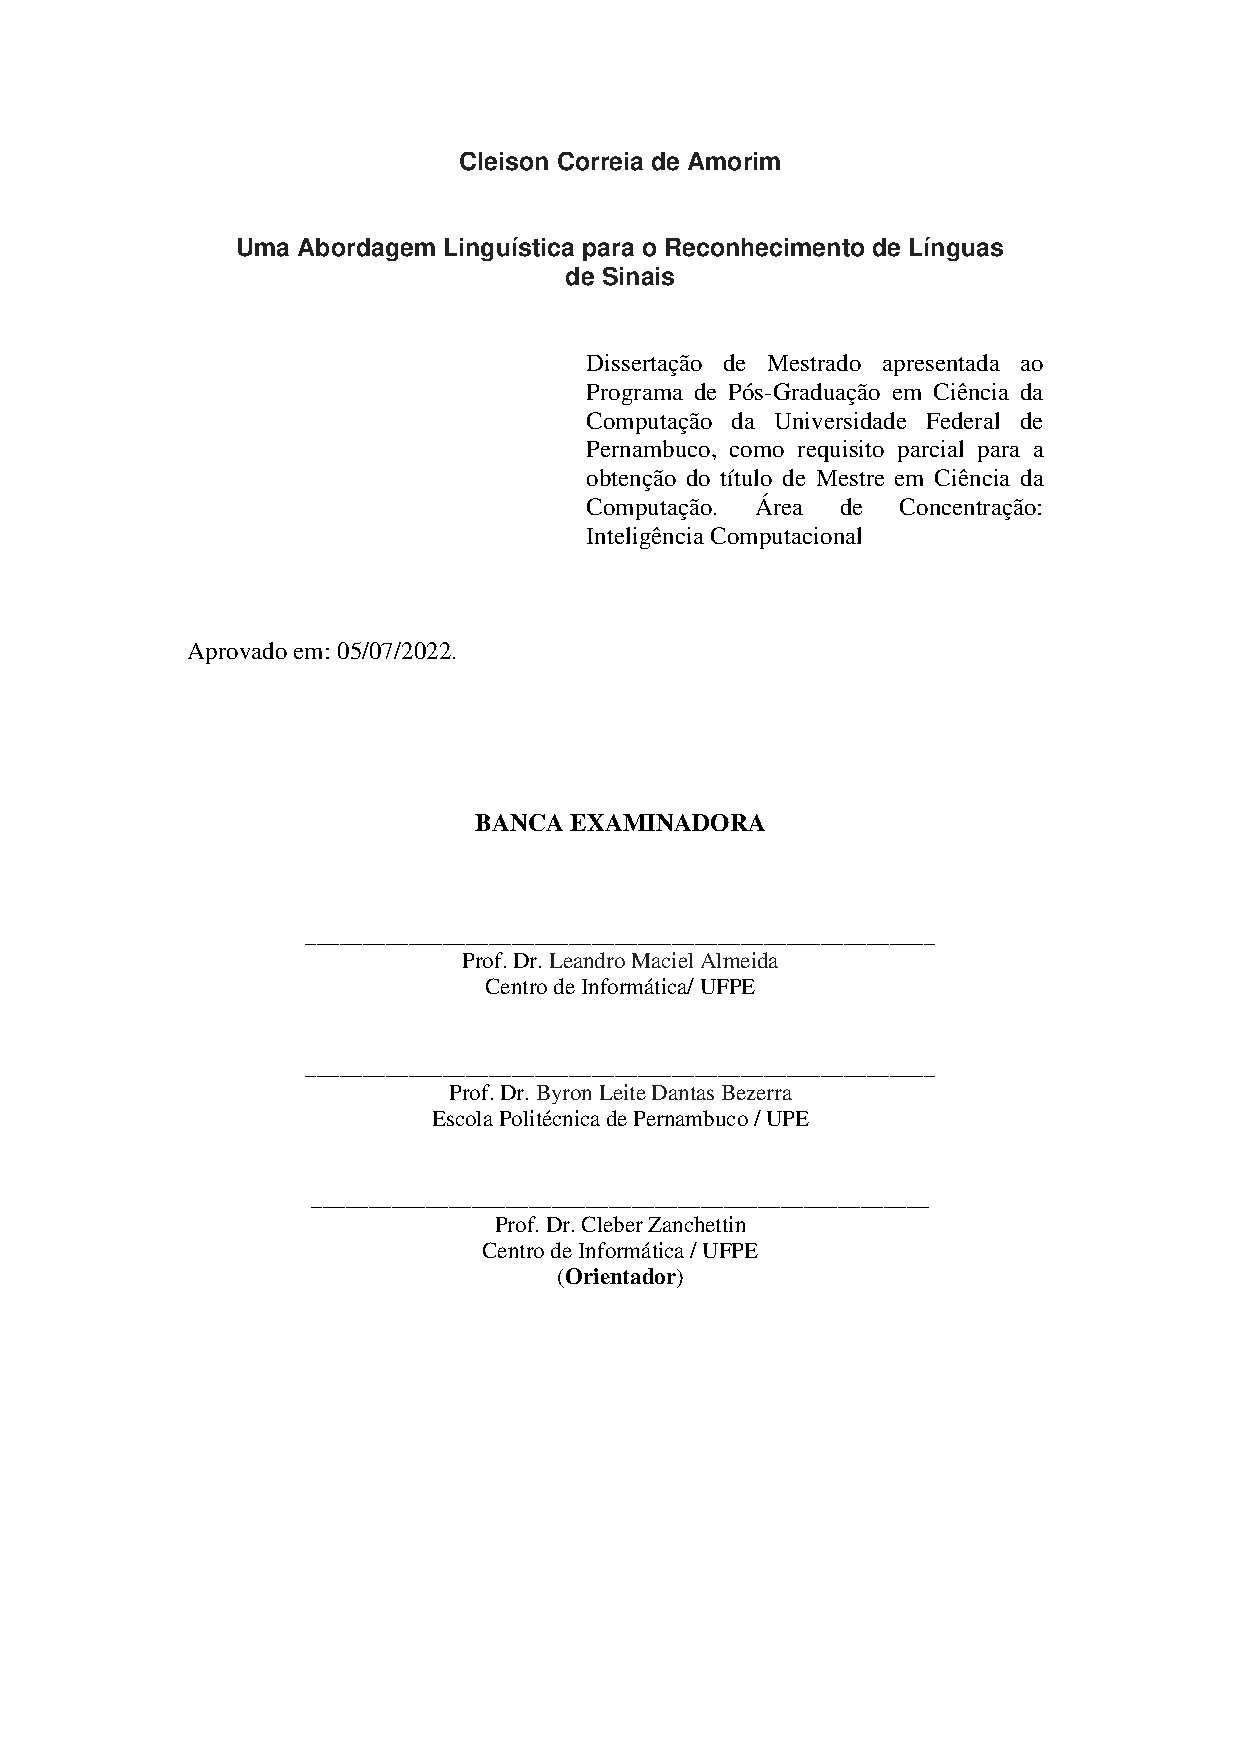
\includepdf[pages=-]{outros/biblioteca/folha_aprovacao}

% ----------------------------------------------------------
% DEDICATÓRIA
% ----------------------------------------------------------
\begin{dedicatoria}
   \vspace*{\fill}
   % \centering
   % \noindent
   \textit{
      Dedico este trabalho ao meu pai, que partiu ao longo da jornada deste mestrado, mas que deixou um grande exemplo de integridade e simplicidade pelo qual me espelharei em minha caminhada.
   }
\end{dedicatoria}
% ---

% ----------------------------------------------------------
% AGRADECIMENTOS
% ----------------------------------------------------------
\begin{agradecimentos}
Texto texto texto texto texto texto texto texto texto texto texto texto texto texto texto texto texto texto texto texto texto texto texto texto texto texto texto texto texto texto texto texto texto texto texto texto texto texto texto texto texto texto.

Texto texto texto texto texto texto texto texto texto texto texto texto texto texto texto texto texto texto texto texto texto texto texto texto texto texto texto texto texto texto texto texto texto texto texto texto texto texto texto texto texto texto.

Texto texto texto texto texto texto texto texto texto texto texto texto texto texto texto texto texto texto texto texto texto texto texto texto texto texto texto texto texto texto texto texto texto texto texto texto texto texto texto texto texto texto.

Texto texto texto texto texto texto texto texto texto texto texto texto texto texto texto texto texto texto texto texto texto texto texto texto texto texto texto texto texto texto texto texto texto texto texto texto texto texto texto texto texto texto.



\end{agradecimentos}
% ----------------------------------------------------------
% EPÍGRAFE

%Epígrafe: Elemento opcional e sem título em que o (a) autor (a) apresenta uma citação relacionada ao assunto tratado no trabalho. Deve ser elaborada conforme a ABNT-NBR 10520 (Citações). As citações de até três linhas devem estar entre aspas duplas e as citações com mais de três linhas devem ser destacadas com recuo de 4 cm da margem esquerda, com letra menor que a do texto e sem as aspas. A fonte da citação deve aparecer na lista de referências.
% ---------------------------------------------------------
\vspace*{\fill}

\begin{citacao}
  ``Conheça todas as teorias, domine todas as técnicas, mas ao tocar uma alma humana seja apenas outra alma humana.''
  (Carl Gustav Jung)
\end{citacao}

\newpage
% -----------------------------------------------------------
% PORTUGUÊS
% -----------------------------------------------------------
\begin{resumo}[Resumo]
  \noindent
  A língua de sinais é uma ferramenta essencial na vida do Surdo, capaz de assegurar seu acesso à comunicação, educação e desenvolvimento cognitivo e socio-emocional.
  Na verdade, ela é a principal força que une essa comunidade e o símbolo de identificação entre seus membros.
  Contudo, atualmente o número de indivíduos ouvintes que conseguem se comunicar por meio dessa língua é pequeno e, na prática, isso impõe obstáculos ao cotidiano do Surdo.
  Tarefas simples como utilizar o transporte público, comprar roupas, ir ao cinema ou obter assistência médica acabam tornando-se um desafio por conta dessa limitação.
  O Reconhecimento de Língua de Sinais é uma das áreas de pesquisa que objetiva desenvolver tecnologias capazes de reduzir essas barreiras linguísticas e facilitar a comunicação entre ambos indivíduos.
  Apesar disso, ao analisar sua evolução ao longo das últimas décadas, percebe-se que seu progresso ainda não é suficiente para disponibilizar soluções efetivamente aplicáveis ao mundo real.
  Isso ocorre principalmente porque várias pesquisas na área acabam não apropriando-se ou abordando adequadamente as particularidades linguísticas das línguas de sinais, decorrentes de sua natureza visual.
  Tendo isso em vista, este trabalho apresenta uma abordagem que aplica modelos sequenciais de aprendizagem de máquina para realizar o reconhecimento computacional dos sinais através de seus atributos linguísticos. Além disso, são introduzidos dois novos \textit{datasets} para a língua de sinais, dentre os quais está um \textit{dataset} de atributos linguísticos computados a partir do ASLLVD.
  Com isso, objetiva-se estabelecer uma direção capaz de conduzir a avanços mais efetivos para essa área e, consequentemente, contribuir com a superação dos obstáculos hoje enfrentados pelo Surdo.

  \vspace{\onelineskip}

  \noindent
  \textbf{Palavras-chaves}: Língua de Sinais. Linguística. Processamento de Linguagem Natural.
\end{resumo}



% -----------------------------------------------------------
% INGLÊS
% -----------------------------------------------------------
\begin{resumo}[Abstract]
  \begin{otherlanguage*}{english}
    \noindent
    Sign language is an essential resource to ensure the Deaf to have access to communication, education, as well as to cognitive and socio-emotional development. In fact, it is the main force that unites such community and the key trait that identifies its members.
    On the other hand, the number of hearing individuals who are able to communicate through this language is currently small and, in practice, this imposes obstacles to the daily life of the Deaf.
    Simple tasks like using public transportation, shopping for clothes, going to the movies, or getting medical assistance end up becoming challenges due to such limitation.
    The Sign Language Recognition, in turn, is one of the research areas dedicated to developing technologies that aim to reduce such language barriers and facilitate the communication between these individuals.
    However, when analyzing its evolution over the last decades, we realize that it has not progressed enough to provide solutions effectively applicable to the real world.
    This is mainly because several researches in this field do not appropriate or address the linguistic particularities presented by the sign languages, which stem from their visual nature.
    Considering this problem, the present work introduces an approach that adopts sequential machine learning models to recognize signs through their linguistic attributes. In addition, we introduce two new sign language datasets, among which is a novel dataset of linguistic attributes computed from the ASLLVD.
    Thus, we aim to establish a direction that can lead to more effective advances in this research area and, consequently, contribute to overcoming the obstacles faced by the Deaf today.

    \vspace{\onelineskip}

    \noindent
    \textbf{Keywords}: Sign Language. Linguistics. Natural Language Processing.
  \end{otherlanguage*}
\end{resumo}



% ----------------------------------------------------------
% LISTA DE FIGURAS
% ----------------------------------------------------------
\pdfbookmark[0]{\listfigurename}{lof}
\listoffigures*
\cleardoublepage


% ----------------------------------------------------------
% LISTA DE CÓDIGOS FONTES
% ----------------------------------------------------------
% define formato e estilo dos elementos do tipo Codigo Fonte
\lstset{
    language=Java,
    basicstyle=\ttfamily\scriptsize,
    %basicstyle=\ttfamily,
    keywordstyle=\color{javapurple}\bfseries,
    stringstyle=\color{pblue},
    commentstyle=\color{javagreen},
    morecomment=[s][\color{javadocblue}]{/**}{*/},
    morecomment=[s][\color{gray}]{@}{\ },
    numbers=left,
    numberstyle=\tiny\color{black},
    backgroundcolor=\color{gray},
    stepnumber=2,
    numbersep=8pt,
    xleftmargin=14pt,
    tabsize=4,
    showspaces=false,
    showstringspaces=false,
    breaklines=true,
}

\pdfbookmark[0]{\lstlistingname}{lol} % caso não tenha código fonte, comente esta linha 
\counterwithout{lstlisting}{chapter}

% Altera o nome padrão do rótulo usado no comando \autoref{}
\renewcommand{\lstlistingname}{Código Fonte}

% Altera o rótulo a ser usando no elemento pré-textual "Lista de código"
\renewcommand{\lstlistlistingname}{Lista de códigos}

% Configura a 'Lista de Códigos' conforme as regras da ABNT (para abnTeX2)
\begingroup\makeatletter
\let\newcounter\@gobble\let\setcounter\@gobbletwo
  \globaldefs\@ne \let\c@loldepth\@ne
  \newlistof{listings}{lol}{\lstlistlistingname}
  \newlistentry{lstlisting}{lol}{0}
\endgroup

\renewcommand{\cftlstlistingaftersnum}{\hfill--\hfil}

\let\oldlstlistoflistings\lstlistoflistings
{
    \let\oldnumberline\numberline
    \newcommand{\algnumberline}[1]{Código Fonte~#1~\enspace--~\enspace}
    \renewcommand{\numberline}{\algnumberline}
    
    \begin{KeepFromToc}
    \lstlistoflistings
    \end{KeepFromToc}
}
\cleardoublepage



% ----------------------------------------------------------
% LISTA DE QUADROS
% ----------------------------------------------------------
\pdfbookmark[0]{\listofquadrosname}{loq} % caso não tenha quadros, comente esta linha 
\listofquadros* % caso não tenha quadros, comente esta linha 
\cleardoublepage



% ----------------------------------------------------------
% LISTA DE TABELAS
% ----------------------------------------------------------
\pdfbookmark[0]{\listtablename}{lot}
\listoftables*
\cleardoublepage


        
  
% ----------------------------------------------------------
% LISTA E ABREVIATURAS E SIGLAS
% ----------------------------------------------------------
%\printglossary[type=\acronymtype,title={\listadesiglasname},nonumberlist]
%\printglossaries
% compile uma vez com o comando \printglossaries e depois compile novamente com o comando \printglossaries comentado para as páginas glossário e siglas serem ocultadas.


% \setglossarystyle{modsuper}
\printnoidxglossary[style=modsuper,type=\acronymtype,title={\listadesiglasname},nonumberlist]
% \printglossary[style=super, type=\acronymtype]
\cleardoublepage



% ----------------------------------------------------------
% LISTA DE SIMBOLOS
% ----------------------------------------------------------
% ---

% ---
% inserir lista de símbolos
% ---
\begin{simbolos}
  \item[$ \gamma $] Letra grega Gama
  %\item[$ \Lambda $] Lambda
  %\item[$ \zeta $] Letra grega minúscula zeta
  \item[$ \in $] Pertence
%  \item[$ \infty$] Infinito
%  \item[$ \ge$] Maior ou Igual
  \item[$ \delta$] Delta
  \item[$ \theta$] Teta
  \item[$ \sigma$] Sigma
  \item[$ \mu$] Mi
  
\end{simbolos}
% ---



% ----------------------------------------------------------
% SUMÁRIO
% ----------------------------------------------------------
\pdfbookmark[0]{\contentsname}{toc}
\tableofcontents*
% \begingroup\intoctrue
% \tableofcontents*
% \endgroup
\cleardoublepage

% \setcounter{page}{13}
\setcounter{tocdepth}{2}
\setcounter{table}{0}



% ----------------------------------------------------------
% ELEMENTOS TEXTUAIS
% ----------------------------------------------------------
\textual
% ===================================================
\chapter{Introdução}
\label{cap-introducao}
\section{Motivação}
\label{motivacao}

% TODO: corrigir 'deficiente auditivo' ??? -- de acordo com PNS (pg 40), é apenas aquele que tem: (1) Muita dificuldade de ouvir ou não consegue de modo algum ouvir
% *** Sugestão ***: Ao modificar para "surdo" x "Surdo", apontar referência:
% "Seguindo convenção proposta por James Woodward (1982), neste livro será  usado o termo “surdo” para se referir à condição audiológica de não ouvir, e o termo “Surdo” para se referir a um grupo particular de pessoas surdas que partilham  uma língua e uma cultura" \cite{pereira-2011-conhecimento-alem-sinais}. 

Segundo a \acrfull{oms}, 19\% da população mundial apresenta algum grau de perda auditiva -- ou seja, em meio a uma população de 7,7 bilhões de habitantes, 1,5 bilhões de indivíduos sofrem com perda auditiva. Dentre esses, 450 milhões referem-se a perda de grau moderado ou severo e que necessitam de acesso a cuidados auditivos e outros serviços de reabilitação -- é o que nos revela o \textit{World Report on Hearing} (Relatório Mundial sobre Audição) publicado em 2021~\cite{who-2021-report-hearing}.

% Conforme o mundo alcança 10 bilhões de habitantes até 2050, a \acrshort{oms} estima que esse 2,5 bilhões de indivíduos (ou 25\% da população mundial) viverão com perda auditiva, dentre os quais 700 milhões serão perda de grau moderado ou severo~\cite{who-2021-report-hearing, opas-2021-oms-estima}.

% O mundo possui hoje 7,7 bilhões de habitantes, dentre os quais 1,5 bilhões de indivíduos possuem perda auditiva (o que equivale a 19\% da população mundial), sendo 450 milhões perda auditiva de moderada ou severa -- é o que aponta a \acrfull{oms} através do seu \textit{World Report on Hearing} (Relatório Mundial sobre Audição) publicado em 2021~\cite{who-2021-report-hearing}.

% Conforme a população mundial cresce para cerca de 10 bilhões de habitantes em 2050, estima-se que 2,5 bilhões de pessoas terão perda auditiva, dentre os quais 700 milhões serão de grau moderado ou elevado e necessitarão de acesso a cuidados auditivos e outros serviços de reabilitação~\cite{who-2021-report-hearing, opas-2021-oms-estima}

No Brasil, o panorama é de 10,7 milhões de habitantes com perda auditiva (ou 5\% da população), dos quais 2,3 milhões correspondem a perda moderada ou severa~\cite{ebc-2019-10-milhoes-pessoas, ibge-2021-pns, ibge-2021-projecao-populacao}. De acordo com o Instituto Locomotiva e o \citeauthor{ibge-2021-pns}, há uma homogeneidade entre homens e mulheres nessa população (54\% homens e 46\% mulheres), mas uma concentração maior nas regiões Sudeste (42\%) e Nordeste (26\%), seguidas pelo Sul (19\%), Norte (7\%) e Centro-Oeste (6\%). Além disso, como a perda auditiva é adquirida ao longo da vida em 91\% dos casos e agrava-se com o passar dos anos, nota-se uma predominância de indivíduos na faixa dos 60 anos de idade ou mais (57\%)~\cite{ebc-2019-10-milhoes-pessoas, ibge-2021-pns}.

Ainda de acordo com a \acrshort{oms}, as últimas décadas testemunharam avanços revolucionários no diagnóstico e reabilitação de problemas auditivos, como no campo da tecnologia auditiva, diagnóstico e telemedicina, com inovações que permitem que perdas e doenças relacionadas à audição sejam identificadas em qualquer idade e ambiente. Gestão médica e cirúrgica, aparelhos auditivos, implantes cocleares, terapia de reabilitação, linguagem de sinais e legendagem são exemplos de soluções que podem garantir que pessoas com doenças de ouvido ou com perda auditiva tenham acesso à educação e comunicação e, assim, tenham a oportunidade de cumprir seu potencial~\cite{who-2021-report-hearing}.

% Ao analisar dispositivos e intervenções capazes de auxiliar no diagnóstico e reabilitação dessas pessoas, a \acrshort{oms} afirma que as últimas décadas testemunharam avanços revolucionários, como no campo da tecnologia auditiva, diagnóstico e telemedicina, com inovações que permitem que perdas e doenças relacionadas à audição sejam identificadas em qualquer idade e ambiente. Gestão médica e cirúrgica, aparelhos auditivos, implantes cocleares, terapia de reabilitação, linguagem de sinais e legendagem são exemplos de soluções que podem garantir que pessoas com doenças de ouvido ou com perda auditiva tenham acesso à educação e comunicação e, assim, tenham a oportunidade de cumprir seu potencial~\cite{who-2021-report-hearing}.


No entanto, há uma disparidade no acesso a esses recursos, uma vez que a grande maioria das pessoas com perda auditiva não consegue acessá-los por viver em locais de baixa renda, onde profissionais especializados e serviços para cuidados auditivos não estão comumente disponíveis~\cite{who-2021-report-hearing}. Segundo a \citeauthor{opas-2021-oms-estima}, 78\% desses países têm menos de um otorrinolaringologista, 93\% têm menos de um audiologista, 83\% têm menos de um fonoaudiólogo, e 50\% têm menos de um professor para deficientes auditivos por milhão de habitantes. Mesmo em países com proporções relativamente altas desses profissionais, há uma distribuição desigual e isso não só representa desafios para as pessoas que precisam de atenção, mas também impõe demandas excessivas aos quadros que prestam esses serviços~\cite{opas-2021-oms-estima}.

%\begin{quote}
%    Entre os países de baixa renda, cerca de 78\% têm menos de um especialista em ouvido, nariz e garganta por milhão de habitantes; 93\% têm menos de um audiologista por milhão; apenas 17\% têm um ou mais fonoaudiólogos por milhão; e 50\% têm um ou mais professores para pessoas com deficiência auditiva por milhão. Mesmo em países com proporções relativamente altas de profissionais de saúde auditiva e de ouvido, há distribuição desigual de especialistas. Isso não só representa desafios para as pessoas que precisam de atenção, mas também impõe demandas excessivas aos quadros que prestam esses serviços~\cite{opas-2021-oms-estima}.
%\end{quote}

Marcos Sarvat, membro da Câmara Técnica de Cirurgia de Cabeça e Pescoço e Otorrinolaringologia do \acrfull{cfm}, ratifica que esse problema na assistência à saúde para deficientes auditivos é acentuado em países subdesenvolvidos, entre os quais está o Brasil. Segundo ele, é difícil o acesso à prevenção por meio de exames periódicos, bem como às consultas, aos medicamentos, às cirurgias e às próteses~\cite{ebc-2021-oms-estima}. Ele destaca ainda que essa falta de cuidados adequados gera deficiências estruturais, que resultam numa pior qualidade de vida que se estende a todas as gerações:

% Marcos Sarvat, membro da Câmara Técnica de Cirurgia de Cabeça e Pescoço e Otorrinolaringologia do \acrfull{cfm}, ratifica que o problema na assistência à saúde para as pessoas com perda de audição é acentuado nos países subdesenvolvidos, entre os quais está o Brasil. Segundo ele, é difícil o acesso à prevenção por meio de exames periódicos, bem como às consultas, aos medicamentos, às cirurgias e às próteses~\cite{ebc-2021-oms-estima}. Ele destaca ainda que essa falta de cuidados adequados à saúde auditiva gera deficiências estruturais, que resultam numa pior qualidade de vida que se estende a todas as gerações:

\begin{citacao}
    {[\dots]} isso reflete na educação das crianças. Uma criança que ouve mal aprende mal e se torna um adulto menos capaz do que seria, e assim por diante. Temos uma cascata de efeitos do idoso abandonado, do idoso solitário, da depressão, da perda de motivação, do desvínculo familiar, da perda de condições de trabalho. Tudo isso vem em cascata e é ignorado~\cite{ebc-2021-oms-estima}.
\end{citacao}

% TODO: revisar 'surdo' aqui:
Reflexos dessas deficiências estruturais são também encontrados na dificuldade de acesso a oportunidades básicas por esses indivíduos, como educação (dados de 2019 mostram que apenas 6\% concluíram o ensino superior; 14\% o ensino médio, 8\% o ensino fundamental e 71\% não possuem grau de instrução) e emprego (apenas 25\% estão no mercado de trabalho)~\cite{ibge-2021-pns}. Além disso, a grande maioria (87\%) não utiliza aparelhos auditivos porque são caros e inacessíveis. Renato Meirelles, que é presidente do Instituto Locomotiva, comenta:

\begin{citacao}
    {[\dots]} como a população surda teve menos oportunidade de estudar do que a população ouvinte; como tem mais dificuldade no mercado de trabalho do que a população ouvinte; o dinheiro para conseguir o aparelho é ainda mais difícil. Esse conjunto de preconceitos que existe na sociedade acaba criando um círculo vicioso que não possibilita que os surdos e os ouvintes tenham as mesmas oportunidades de se dar bem na vida~\cite{ebc-2019-10-milhoes-pessoas}.
\end{citacao}


Em meio a esses desafios que limitam o acesso aos cuidados e tecnologias adequados para reabilitação desses indivíduos, a língua de sinais acaba sobressaindo-se como uma alternativa que é mais inclusiva -- isso porque impõe menos barreiras ao não demandar investimento financeiro elevado ou a disponibilidade de profissionais especializados no serviço público de saúde pelo país. Apesar disso, ela é capaz de assegurar o desenvolvimento cognitivo, facilitar a comunicação, e possibilitar que crianças com deficiência auditiva obtenham educação e desenvolvimento socio-emocional adequado~\cite{who-2021-report-hearing}. % TODO: adicionar mais aqui
É possível aprender línguas de sinais por meio da própria família, da comunidade surda ou de recursos como livros, cursos, vídeos e materiais disponibilizados muitas vezes gratuitamente pela internet ou em escolas da rede pública de educação e institutos de surdos -- entre os quais o \acrfull{ines} é talvez o mais antigo, fundado em 1857~\cite{pereira-2011-conhecimento-alem-sinais}. 


% é capaz de assegurar o desenvolvimento cognitivo, facilitar a comunicação, e possibilitar que crianças obtenham educação e desenvolvimento socio-emocional adequado~\cite{who-2021-report-hearing}. Ela torna-se mais acessível porque não demanda investimento financeiro elevado ou que profissionais especializados estejam disponíveis de forma igualitária sobretudo no serviço público de saúde pelo país -- é possível aprender a língua de sinais através da própria família, da comunidade surda ou por meio de cursos, livros e outros recursos disponibilizados de forma gratuita na internet, em escolas públicas ou em institutos de surdos -- como o \acrfull{ines}, em funcionamento desde 1857~\cite{pereira-2011-conhecimento-alem-sinais}.

No Brasil, a língua sinalizada oficial é a \acrfull{libras}, a que foi reconhecida como meio legal de comunicação e expressão pela Lei n° 10.436, de 24 de abril de 2002~\cite{brasil-2002-lei10436}. Através dessa lei, a língua passou a receber maior atenção por educadores e pesquisadores, fazendo crescer significativamente o número de adeptos e defensores de sua utilização~\cite{pereira-2011-conhecimento-alem-sinais}.

% TODO: revisar se há contradição aqui:
% No entanto, apesar do papel fundamental que essa língua é capaz de exercer na comunicação do deficiente auditivo, dados do \acrshort{ibge} revelam que nem todos esses indivíduos a conhecem -- no Brasil, apenas 13\% dos que possuem perda auditiva moderada e 61\% daqueles com perda severa conhecem a \acrshort{libras}~\cite{ibge-2021-pns}. Apesar de não haver um análise concreta das razões que conduzem a isso, pode-se enumerar alguns motivos que contribuem para tal: uma vez que a perda auditiva é adquirida ao longo da vida em 91\% dos casos e, muitos desses indivíduos já são oralizados e usuários do português, eles preferem continuar utilizando a própria fala (auxiliados por dispositivos auditivos ou implantes cocleares) ou adotar a leitura labial; em outra parcela, há resistência de muitos pais de crianças que nascem surdas ou perdem a audição muito cedo, os quais rejeitam a língua de sinais e impõem a oralização de seus filhos; por fim, pode haver ainda um deficit ao incorporar e preparar os professores para o ensino da \acrshort{libras} como parte da currículo regular, fazendo com que muitas indivíduos concluam seus estudos como analfabetos funcionais~\cite{lobato-2021-surdez-nao-sinonimo-libras, ebc-2019-10-milhoes-pessoas, senado-2019-baixo-alcance-lingua-sinais}.


Se por um lado a língua de sinais é uma poderosa ferramenta que permite a comunicação e o desenvolvimento cognitivo do deficiente auditivo; por outro lado ainda há um obstáculo relevante que os distancia de uma plena inclusão em sociedade: a escassez de ouvintes que conhecem a língua de sinais e conseguem se comunicam por meio dela~\cite{bragg-2019-slr-interdisciplinary}. De acordo com a \citeauthor{senado-2019-baixo-alcance-lingua-sinais}, a língua de sinais está restrita à comunidade surda e isso transforma atividades corriqueiras num grande desafio, levando eles ao isolamento. No transporte público, por exemplo, esses indivíduos não conseguem pedir ajuda, requisitar informações sobre as rotas ou ter acesso aos anúncios nos alto-falantes sobre mudanças nelas; no cinema, eles não podem assistir filmes nacionais, pois apenas filmes estrangeiros dispõem de legendas; em lojas, é raro encontrar vendedores preparados para interagir em língua de sinais; no serviço de saúde, os surdos perdem sua vez se não estiverem atentos à enfermeira que fala o nome do próximo paciente, além de estarem suscetíveis a situações ainda mais trágicas: ONGs dedicadas aos surdos afirmam que não são raros os casos em que pacientes saem de consultas com uma prescrição errada de medicamento porque o médico não entendeu quais eram os sintomas; no mercado de trabalho, é comum empresas contratarem esses indivíduos para cumprir as cotas exigidas em lei, mas não se preocuparem em saber como eles são -- eles são muitas vezes vistos como incapazes e são designados a tarefas secundárias~\cite{senado-2019-baixo-alcance-lingua-sinais}.


% Apesar disso, os surdos ainda estão longe de uma plena inclusão na sociedade: o grande obstáculo é a escassez de ouvintes que se comuniquem na língua de sinais. De acordo com a \citeauthor{senado-2019-baixo-alcance-lingua-sinais}, a \acrshort{libras} está restrita à comunidade surda e isso transforma atividades corriqueiras num grande desafio, levando o surdo ao isolamento. No transporte público, por exemplo, esses indivíduos não conseguem pedir ajuda, requisitar informações sobre as rotas ou ter acesso aos anúncios nos alto-falantes sobre mudanças nelas; no cinema, eles não podem assistir filmes nacionais, pois apenas filmes estrangeiros dispõem de legendas; em lojas, não é difícil encontrar vendedores despreparados para interagir em língua de sinais ou que demonstrem preconceito com esses indivíduos; no serviço de saúde, os surdos perdem vez se não estiverem atentos à enfermeira que chama o nome do próximo paciente e estão suscetíveis a situações que podem ser ainda mais trágicas: ONGs dedicadas aos surdos afirmam que não são raros os casos em que pacientes com problemas sérios de saúde saem de consultas com uma prescrição errada de remédio, porque o médico não entendeu quais eram os sintomas; no mercado de trabalho, é comum empresas contratarem os surdos para cumprir as cotas exigidas em lei, mas não se preocuparem em saber como eles são -- elas encaram os surdos como incapazes e os atribuem tarefas secundárias~\cite{senado-2019-baixo-alcance-lingua-sinais}.

Um passo importante para contribuir com a quebra dessas barreiras consiste na pesquisa e desenvolvimento de tecnologias de processamento de língua de sinais -- que inclui o reconhecimento, geração e tradução dessa língua. 
Por meio delas, é possível conectar usuários e não-usuários da língua sinalizada, provendo assistência à sua comunicação e permitindo que a mensagem seja compreendida pelos interlocutores independentemente da barreira linguística -- semelhante ao que se observa para diálogos envolvendo línguas não-visuais de nacionalidades distintas.
Segundo \citeauthor{bragg-2019-slr-interdisciplinary}, essas tecnologias também tornariam acessíveis aos usuários dessa língua recursos úteis ao nosso cotidiano e que ainda não estão disponíveis para eles, como os assistentes pessoais, que são limitados ao uso de comandos de voz e que poderiam passar a responder pessoas articulando sinais. Além disso, a tradução dos sinais para texto poderia permitir o uso de mecanismos de busca ou outros sistemas baseados em texto de uma forma mais amigável; o processo inverso, por sua vez, poderia substituir automaticamente conteúdo textual por animações em língua de sinais. Outras possibilidades incluiriam a transcrição automática de vídeos produzidos em língua de sinais -- o que permitiria, por exemplo, uma indexação e busca desse conteúdo; a interpretação em tempo real quando não há intérpretes humanos disponíveis; ou outras ferramentas e aplicativos educacionais~\cite{bragg-2019-slr-interdisciplinary}.


% These technologies would make voice-activated services newly accessible to deaf sign language users – for example, enabling the use of personal assistants (e.g., Siri and Alexa) by training them to respond to people signing. They would also enable the use of text-based systems – for example by translating signed content into written queries for a search engine, or automatically replacing displayed text with sign language videos. Other possibilities include automatic transcription of signed content, which would enable indexing and search of sign language videos, real-time interpreting when human interpreters are not available, and many educational tools and applications.

% reconhecimento, tradução e transcrição dessa língua para outros idiomas (e de outros idiomas para ela). Em sua essência, essas tecnologias visam prover assistência nessa comunicação permitindo que esses indivíduos compreendam-se mutuamente mesmo utilizando línguas distintas. É uma tarefa desafiadora que tem sido abordada de forma multidisciplinar no decorrer das últimas décadas por diferentes subáreas da Ciência da Computação. \cite{bragg-2019-slr-interdisciplinary}

% Um passo importante para contribuir com a quebra dessas barreiras consiste na pesquisa e desenvolvimento de tecnologias para o reconhecimento, tradução e transcrição dessa língua para outros idiomas (e de outros idiomas para ela). Em sua essência, essas tecnologias visam prover assistência nessa comunicação permitindo que esses indivíduos compreendam-se mutuamente mesmo utilizando línguas distintas. É uma tarefa desafiadora que tem sido abordada de forma multidisciplinar no decorrer das últimas décadas por diferentes subáreas da Ciência da Computação. \cite{bragg-2019-slr-interdisciplinary}



% Um passo importante para redução dessas barreiras na comunicação entre usuários e não-usuários da língua sinalizada compreende a pesquisa e desenvolvimento de tecnologias capazes de realizar o reconhecimento, tradução e transcrição dessa língua para outros idiomas e vice-versa. Essa é uma tarefa desafiadora que vem sendo abordada de forma multidisciplinar no decorrer das últimas décadas por subáreas da Ciência da Computação -- a exemplo do \acrfull{slr}, que aplica reconhecimento de padrões, visão computacional, processamento de linguagem natural e linguística para construir métodos e algoritmos objetivam identificar sinais produzidos e compreender seu significado~\cite{wadhawan-2021-slr-systems-review}.

% TODO: revisar se SLR deveria ser especificado aqui (ou falar de forma mais abrangente das pesquisas)
O \acrfull{slr} é uma das áreas de pesquisa empenhadas em contribuir para que tecnologias como essas sejam desenvolvidas. Trata-se de uma área colaborativa que envolve reconhecimento de padrões, visão computacional, processamento de linguagem natural e linguística para construir métodos e algoritmos capazes de identificar sinais produzidos e compreender seu significado~\cite{wadhawan-2021-slr-systems-review}. 
Apesar disso, \citeauthor{cooper-2011-slr} acreditam que o progresso apresentado por ela nas últimas décadas ainda foi pouco expressivo:

\begin{citacao}
    Enquanto sistemas de reconhecimento automático da fala avançaram ao ponto de estarem comercialmente disponíveis, o reconhecimento de sinais ainda está em sua infância. Atualmente, todos os serviços comerciais de tradução de sinais são baseados em humanos e requerem pessoal especializado -- o que os tornam caros~\cite[tradução nossa]{cooper-2011-slr}.
\end{citacao}

% \citeauthor{bragg-2019-slr-interdisciplinary} argumentam que 
%Current research in sign language processing occurs in disciplinary silos, and as a result does not address the problem comprehensively. For example, there are many computer science publications presenting algorithms for recognizing (and less frequently translating) signed content. The teams creating these algorithms often lack Deaf members with lived experience of the problems the technology could or should solve, and lack knowledge of the linguistic complexities of the language for which their algorithms must account. The algorithms are also often trained on datasets that do not reflect real-world use cases. As a result, such single-disciplinary approaches to sign language processing have limited real-world value [39].
%To overcome these problems, we argue for an interdisciplinary approach to sign language processing. Deaf studies must be included in order to understand the community that the technology is built to serve. Linguistics is essential for identifying the structures of sign languages that algorithms must handle. Natural Language Processing (NLP) and machine translation (MT) provide powerful methods for modeling, analyzing, and translating. Computer vision is required for detecting signed content, and computer graphics are required for generating signed content. Finally, Human-Computer Interaction (HCI) and design are essential for creating end-to-end systems that meet the community's needs and integrate into people's lives.

% Os autores acreditam que parte disso deve-se ao fato de que muitas pesquisas em \acrshort{slr} abordam o problema de forma incorreta: eles encaram o reconhecimento da língua de sinais como uma tarefa de reconhecimento de gestos, concentrando-se na identificação de características e métodos para rotular um sinal dentre um conjunto de possibilidades bem definidas -- porém, essas línguas vão muito além disso.


\citeauthor{bragg-2019-slr-interdisciplinary} e \citeauthor{cooper-2011-slr} acreditam que, de uma forma geral, isso está relacionado a fatores como os desafios particulares a essas línguas e a forma com que as pesquisas desenvolvidas na área têm abordando o problema no decorrer das últimas décadas.
Pode-se sumarizar esses fatores nos seguintes itens principais:

\begin{enumerate}
    % TODO: revisar esse contraponto ao reconhecimento da lingua de sinais
    \item Abordagem inadequada do problema: pesquisas atuais em processamento de língua de sinais ocorrem em silos disciplinares e, como resultado, não abordam o problema de uma forma holística. Por exemplo, muitas delas abordam o reconhecimento, mas poucas contemplam a tradução dos sinais em contextos reais ou consideram elementos como a linguística nesse processo.
    Há ainda pesquisas que abordam o problema como uma tarefa de reconhecimento de gestos e buscam identificar métodos para rotular um sinal dentre um conjunto de possibilidades bem definidas -- no entanto, essas línguas vão mais além do que uma coleção de gestos bem definidos.

    \item Natureza multicanal: línguas de sinais transmitem significado através de múltiplos canais ao mesmo tempo -- como por exemplo, a interação entre as mãos, a interação delas para com o corpo do interlocutor, suas orientações e configurações enquanto se movem, as expressões da face, olhos, cabeça e ombros, a intensidade com eles são articulados, entre outros que são abordados na linguística e que ocorrem simultaneamente.
    Isso significa que observar um canal isolado -- como observa-se em muitas pesquisas que contemplam apenas mãos estáticas ou fora do contexto -- é insuficiente para abordar corretamente a língua.
    
    \item Linguística particular: a linguística das línguas sinalizadas nos evidencia que elas possuem diversas particularidades atreladas à sua natureza visual, e isso torna muitas das técnicas hoje utilizadas no processamento das línguas faladas inadequadas a esse contexto.
    Sendo assim, ao invés de reproduzir técnicas empregadas às línguas faladas, é necessário que pesquisas em processamento de línguas sinalizadas desenvolvam técnicas próprias que explorem tais particularidades linguísticas e, com isso, que sejam capazes de contribuir avanços relevantes à área.
    %\item Linguística particular: já é evidente através dos estudos da linguística das línguas sinalizadas que suas particularidades enquanto línguas visuais tornam muitas das técnicas utilizadas para reconhecimento da fala inadequadas para o \acrshort{slr}. Dessa forma, não é correto simplesmente reproduzir abordagens de processamento de fala; mas é preciso compreender e desenvolver técnicas que levem em consideração tais particularidades.
    
    \item \textit{Datasets} limitados: os \textit{datasets} de língua de sinais disponíveis publicamente são limitados em quantidade e qualidade, e isso impõe um desafio relevante para as pesquisas na área. Técnicas modernas de aprendizagem de máquina demandam uma quantidade crescente de dados que representem o contexto de aplicação no mundo real. A escassez desses dados faz que os algoritmos desenvolvidos não sejam capazes de aprender corretamente sobre o domínio do problema e, consequentemente, não sejam capazes de generalizar soluções úteis para o mundo real.
    
\end{enumerate}


Tendo em vista essas lacunas, bem como os papel importante que as línguas de sinais podem desempenhar para auxiliar o deficiente auditivo a superar muitas das barreiras discutidas até aqui, este trabalho contribui introduzindo uma nova abordagem de processamento de sinais que considera a linguística dessas línguas e, consequentemente, sua natureza multicanal para realizar o processamento dos sinais. Além disso, aqui também são apresentados dois novos \textit{datasets} que podem suportar novas pesquisas a continuar evoluindo nessa direção.

%desafios encarados pelos deficientes visuais que foram apresentados até aqui, bem como encarados e o importante papel que as línguas de sinais podem desempenhar para auxiliar os deficientes auditivos a superar muitas dessas barreiras, esse trabalho introduz uma abordagem baseada na linguística para o processamento de línguas de sinais, bem como dois novos \textit{datasets} que visam contribuir com diversas outras pesquisas na área.




% Many approaches to SLR incorrectly treat the problem as Gesture Recognition (GR). So research has thus far focused on identifying optimal features and classification methods to correctly label a given sign from a set of possible signs. However, sign language is far more than just a collection of well specified gestures.
% Sign languages pose the challenge that they are multi-channel; conveying meaning through many modes at once. While the studies of sign language linguistics are still in their early stages, it is already apparent that this makes many of the techniques used by speech recognition unsuitable for SLR. In addition, publicly available data sets are limited both in quantity and quality, rendering many traditional computer vision learning algorithms inadequate for the task of building classifiers.
% However, even given the lack of translation tools, most public services are not translated into sign. There is no commonly-used, written form of sign language, so all written communication is in the local spoken language



% The use of computational approaches to help the learning, communication, translation, and interaction using sign language is essential to include this population in society. In the machine learning research area, Sign Language Recognition (SLR) refers to a collaborative field that involves pattern matching, computer vision, natural language processing, and linguistics [2] to enable sign language users to communicate with spoken languages users. However, while speech recognition systems have advanced to the point of being commercially available, SLR systems are still in very early stages. Therefore, commercial translation services for sign languages are human-based, require specialized personnel, and are often expensive [3].
% Among the main challenges involved, there is the scarcity of approaches structured around the linguistics of the sign language, the limitation in quantity and quality of public datasets that could lead to significant advancements of the SLR techniques, and the multi-channel nature of the language – which convey meaning through many modes at once [3].





% \cite{cooper-2011-slr}:
% While automatic speech recognition has now advanced to the point of being commercially available, automatic SLR is still in its infancy. Currently all commercial translation services are human based, and therefore expensive, due to the experienced personnel required.
% SLR aims to develop algorithms and methods to correctly identify a sequence of produced signs and to understand their meaning. Many approaches to SLR incorrectly treat the problem as Gesture Recognition (GR). So research has thus far focused on identifying optimal features and classification methods to correctly label a given sign from a set of possible signs. However, sign language is far more than just a collection of well specified gestures.
% Sign languages pose the challenge that they are multi-channel; conveying meaning through many modes at once. While the studies of sign language linguistics are still in their early stages, it is already apparent that this makes many of the techniques used by speech recognition unsuitable for SLR. In addition, publicly available data sets are limited both in quantity and quality, rendering many traditional computer vision learning algorithms inadequate for the task of building classifiers.
% However, even given the lack of translation tools, most public services are not translated into sign. There is no commonly-used, written form of sign language, so all written communication is in the local spoken language.


% \cite{wadhawan-2021-slr-systems-review}:
% Sign language recognition is a collaborative research area which involves pattern matching, computer vision, natural language processing, and linguistics. Its objective is to build various methods and algorithms in order to identify already produced signs and to perceive their meaning. Sign language recognition systems are Human Computer Interaction (HCI) based systems that are designed to enable effective and engaging interaction. These system follows a multidisciplinary approach of data acquisition, SL technology, SL testing and SL linguistics. Such a system can be deployed in public services like hotels, railways, resorts, banks, offices etc. to enable hearing impaired people learn new concepts and facts and to control emotional behavior [1].







% =======
% Baixo alcance da língua de sinais leva surdos ao isolamento
% https://www12.senado.leg.br/noticias/especiais/especial-cidadania/baixo-alcance-da-lingua-de-sinais-leva-surdos-ao-isolamento
% Fonte: Agência Senado
% -------
% Em 2002, a Lei 10.436 deu à Libras o status de meio legal de comunicação e expressão. Desde então, escolas, faculdades, repartições do governo e empresas concessionárias de serviços públicos estão obrigadas a providenciar intérpretes para atender aos surdos. A lei faz aniversário em 24 de abril, que, por isso, transformou-se no Dia Nacional da Língua Brasileira de Sinais.
% ------
% Apesar da lei de 2002, os surdos ainda estão longe da plena inclusão na sociedade. Como o curta Libras É Merda? denuncia (às avessas), o grande obstáculo é a escassez de ouvintes que se comuniquem na língua de sinais. A Libras está restrita à comunidade surda. Isso pode transformar atividades corriqueiras num inferno. No ônibus, os surdos não conseguem saber do cobrador qual é a parada em que devem descer. Se o alto-falante do aeroporto anuncia troca de portão, eles correm o risco de perder o avião caso não estejam com os olhos grudados nos telões de voos.
% No cinema, não podem ver filmes nacionais, pois só os estrangeiros são legendados. Na loja, o vendedor menos paciente e esclarecido pode confundir os gestos da língua de sinais com brincadeira ou deficiência mental e simplesmente virar as costas para os clientes surdos.
% Nos serviços de saúde, os surdos perdem a vez quando não estão atentos à enfermeira que grita o nome do próximo paciente. Essa dificuldade, aliás, levou à criação de um projeto-piloto no Sistema Único de Saúde (SUS): o Hospital Federal de Ipanema, no Rio de Janeiro, abriu uma central de atendimento e consulta mediada por intérprete de Libras.
% -----
% As situações podem inclusive ser trágicas. ONGs dedicadas aos surdos dizem que não são raros os casos em que pacientes com problemas sérios de saúde saem de consultas com uma prescrição errada de remédio, porque o médico não entendeu quais eram os sintomas, e situações em que inocentes são mortos porque não ouviram a ordem de parar e o policial atirou por não perceber que eram surdos.
% "Deficiente não é o surdo, mas a sociedade que não sabe se comunicar com ele. Se o surdo encontrasse no dia a dia pessoas que soubessem a língua de sinais, ele não enfrentaria tantas barreiras e, por isso, nem perceberia a surdez como deficiência" afirma a coordenadora do Laboratório de Educação de Surdos e Libras, da Universidade de Brasília (UnB), Edeilce Buzar.
% Segundo o Censo mais recente, viviam em 2010 no Brasil 2,1 milhões de pessoas que escutavam muito pouco ou nada — o equivalente à população de Manaus. A pesquisa do IBGE não apontou quantas faziam uso da língua de sinais.

% CENSO - IBGE 2018:
% - 5% (9,6 milhões) da população brasileira têm deficiência auditiva
% - 2,1 milhões são surdos ou escutam muito pouco
% - 7,5 milhões apresentam alguma dificuldade para ouvir
% - 360 milhões de pessoas sofrem algum tipo de surdez no mundo
% - 32 milhões são crianças
% - 31 milhões vivem em países em desenvolvimento

% As primeiras barreiras linguísticas por vezes são impostas pela própria família. Quando a criança nasce surda ou perde a audição ainda pequena, muitos pais rejeitam a língua de sinais e impõem a oralização. Sem ouvir a própria voz, o treinamento da fala e da leitura labial costuma ser lento e penoso. O aprendizado da língua de sinais, ao contrário, é natural para quem, compensando a lacuna da audição, tem na visão o sentido mais apurado.
% -----
% Raras escolas estão adaptadas para receber alunos surdos. A mera presença de um intérprete da língua de sinais ao lado do professor não é suficiente. Por um lado, muitas crianças surdas chegam ao colégio sem saber língua nenhuma e vão ter que aprender a Libras do zero. Por outro, as que já sabem a língua de sinais não encontram professores preparados para ensinar-lhes o português escrito. Nessa situação, como a Libras é a primeira língua do estudante, o português precisa ser apresentado como segundo idioma, com uma metodologia completamente diferente, tal como uma língua estrangeira. O professor precisa ser bilíngue e ter uma formação específica.
% Em consequência do despreparo das escolas, muitos surdos chegam ao fim dos estudos como analfabetos funcionais. É por isso, aliás, que tentar se comunicar por escrito com um surdo nem sempre dá certo.

% — Os surdos acabam sendo forçados a viver encapsulados em seus próprios mundos. São como almas que passam por nós sem que nos preocupemos em enxergá-los ou interagir com eles — compara o intérprete de Libras e ex-presidente da Associação de Pais e Amigos dos Deficientes Auditivos do Distrito Federal (Apada-DF) Marcos de Brito.
% -----
% Desde 1991, a Lei 8.213 obriga as empresas a reservar uma parte de suas vagas para funcionários com algum tipo de deficiência. Para firmas que tenham entre 100 e 200 trabalhadores, por exemplo, a cota é de 2%. A inclusão efetiva nem sempre ocorre. Tarcísio Barroso, de 31 anos, ficou surdo ainda bebê, também por causa da meningite. Ele é oralizado, mas tem a Libras como primeira língua. Mesmo pós-graduado na área da tecnologia da informação, acabou sendo relegado a tarefas secundárias em muitas das empresas onde trabalhou, em Brasília.
% — A comunicação com meus chefes sempre foi falha. Alguns não se preocupavam em articular bem as palavras na hora de falar, para eu fazer a leitura labial. Outros preferiam se comunicar por escrito, mas usavam palavras difíceis ou frases pouco objetivas, o que dificultava a minha compreensão. De tanto eu pedir que explicassem novamente cada orientação, acabavam concluindo que eu tinha deficiência intelectual e passavam a me deixar de lado. Já chorei muito por causa disso.
% A mãe dele, Vanilda Barroso, lembra que a inadequação que ele agora sente no trabalho é muito parecida com a que sentia no colégio, quando os professores não exploravam as suas potencialidades e só apontavam as dificuldades.
% — As empresas contratam um surdo e nem se preocupam em saber como os surdos são. Só querem cumprir a cota exigida pela lei. Não estão interessadas na inclusão — ela afirma. — E a inclusão não é difícil. Bastaria que as empresas deixassem de encarar o surdo como um incapaz e passassem a vê-lo como um estrangeiro que não compreende plenamente o português e precisa de explicações numa linguagem mais clara.



% ==============
% IBGE confirma: surdez não é sinônimo de Libras
% https://desculpenaoouvi.com.br/ibge-confirma-surdez-nao-e-sinonimo-de-libras/?fbclid=IwAR1Z5mcQeTlaaVCuEtDXDQoLW9cwT17yBplyQUgFF7NXxM7qT5saMTjFaWk
% 
% IBGE - Pesquisa Nacional de Saúde (PNS) - 2019:
% - 8,4% (17,3 milhões) da população com 2+ anos com algum grau de deficiência
%
% Com deficiência auditiva:
% - 1,3% da população em idade de trabalhar (14+ anos)
% - 2,6% da população fora da força de trabalho
%
% Nível de ocupação: 
% - 25,4% das pessoas de 14+ anos
% 
% Nível de instrução (pessoas com 18+ anos): 
% - 67,6% sem instrução e fundamental incompleto
% - 10,8% fundamental completo e médio incompleto
% - 16,6% médio completo e superior incompleto
% - 5% superior completo
%
% Uso de tecnologias auditivas:
% - 0,8% da população 2+ anos
% - 3,1% da população 60+ anos
%
% Uso da Libras (população 5+ anos) por grau de dificuldade para ouvir
% - Alguma dificuldade: 1,8% sabe usar
% - Muita dificuldade: 3,0% sabe usar
% - Não consegue de modo algum: 35,8% sabe usar
% --> "com deficiência auditiva" (grande dificuldade + não consegue de modo algum): 22,4%

% “Além disso, a informação [PNS] é importante para não generalizar as pessoas com deficiência auditiva: ao analisar os dados, é possível perceber que nem todos sabem se comunicar em Libras, pois fazem uso da fala, se comunicam oralmente, muitos deles com o apoio da leitura labial. Portanto, precisam de outros recursos de acessibilidade, como por exemplo as legendas, além de necessitarem de propostas educacionais distintas”, diz a pesquisadora.
% Comprovadamente, acessibilidade para surdos não se resume à interpretação em Libras e, como mostrado pelo IBGE, não atende a necessidade da maioria.

% -----
% Esses dados são essenciais para que se desmistifique que surdez é sinônimo de ser usuário exclusivo da Libras. A Libras tem função fundamental na comunicação de uma parcela de pessoas Surdas, assim como a Língua Portuguesa também tem função fundamental para a grande maioria das pessoas com deficiência auditiva.
% -----
% Não podemos continuar com políticas como as que vêm sendo implementadas nos últimos 10 anos, onde a iniciativa pública e privada decidem erroneamente que basta incluir Libras e todos os surdos serão contemplados com ela.
% -----
% Graças à Pesquisa Nacional de Saúde de 2019 realizada pelo IBGE, podemos afirmar categoricamente que A SURDEZ É PLURAL e as formas de acessibilidade também devem ser.



% =====
% Painel de Indicadores de Saúde – Pesquisa Nacional de Saúde
% https://www.pns.icict.fiocruz.br/painel-de-indicadores-mobile-desktop/


% =====
% País tem 10,7 milhões de pessoas com deficiência auditiva, diz estudo
% https://agenciabrasil.ebc.com.br/geral/noticia/2019-10/brasil-tem-107-milhoes-de-deficientes-auditivos-diz-estudo
% ------

% Instituto Locomotiva + Semana da Acessibilidade Surda:
% - 10,7 milhões de pessoas com deficiência auditiva (Brasil)
%    - Dessas, 2,3 milhões têm deficiência severa
%       - 15% já nasceram surdos
%
% - A surdez atinge 54% de homens e 46% de mulheres
% - A predominância (57%) é na faixa de 60+ anos
% 
% Condição nascida x adquirida:
% - 9% das pessoas nasceram 
% - 91% adquiriram ao longo da vida (metade foi antes dos 50 anos)
% 
% Do total pesquisado:
% - 87% não usam aparelhos auditivos (13% utilizam)

% ------
% “A deficiência auditiva é uma deficiência que se agrava com o passar dos anos. E como o Brasil está passando por um processo de envelhecimento da população, hoje já temos 59 milhões de brasileiros com mais de 50 anos e, em 2050, vamos chegar com mais de 98 milhões de brasileiros com mais de 50 anos de idade, essa é uma tendência que só vai crescer”, disse Renato Meirelles, presidente do Instituto Locomotiva. Completou que a “sociedade, claramente, não está preparada para isso”.

% ------
% Dois em cada três brasileiros 
% - 66,6% relataram enfrentar dificuldades nas atividades do cotidiano
% --> “Com isso, eles se divertem menos, têm menos chance no mercado de trabalho, não têm as mesmas oportunidades educacionais que os ouvintes têm”. 
% -----
% A falta de acolhimento e inclusão limitam o acesso dos surdos às oportunidades básicas, como educação
% - somente 7% têm ensino superior completo
% - 15% frequentaram até o ensino médio
% - 46% até o fundamental
% - 32% não possuem grau de instrução
% -------
% - 20% das pessoas com deficiência auditiva idosos não conseguem sair sozinhas
% - 37% estão no mercado de trabalho
% - 87% não usam aparelhos auditivos
% --> “Porque é muito caro e inacessível para a maioria dessa população”, disse Meirelles. “E como a população surda teve menos oportunidade de estudar do que a população ouvinte, como tem mais dificuldade no mercado de trabalho do que a população ouvinte, o dinheiro para conseguir o aparelho é ainda mais difícil. Esse conjunto de preconceitos que existe na sociedade acaba criando um círculo vicioso que não possibilita que os surdos e os ouvintes tenham as mesmas oportunidades de se dar bem na vida.”
% --> “Quando comecei no meu trabalho, as pessoas pensavam que eu não era capaz de fazer as coisas. Demorou demais para que elas acreditassem que eu tinha capacidades, mas às vezes ainda me olham com discriminação e desconfiança por eu ser quem sou”, afirmou uma mulher com deficiência auditiva de 30 anos, entrevistada em São Paulo.

% ------
% Entre os tipos de ocupação desempenhada pelas pessoas com deficiência auditiva com 18+ anos:
% - 43% empregado no setor privado 
% - 37% trabalhador por conta própria
%
% Segundo Renato Meirelles, “essas pessoas desistiram de arrumar emprego e passaram a empreender para garantir o seu sustento”.
% A pesquisa foi realizada entre os dias 1º e 5 de setembro passado, com 1,5 mil brasileiros surdos e ouvintes. No total, o Brasil possui 50,3 milhões de pessoas com deficiência. 

% -----
% A pesquisa mostra que a maior parcela de pessoas com deficiência auditiva está:
% - 42%: Região Sudeste
% - 26%: Nordeste 
% - 19%: Sul
% - 6%: Centro-Oeste 
% - 7%: Norte

% Das pessoas com deficiência auditiva:
% - 28% declararam ter também algum tipo de deficiência visual
% - 2% deficiência intelectual.

% Dos brasileiros com problemas auditivos:
% 14% não se sentem à vontade e poder falar sobre quase tudo com a família (11% da população de forma geral)
% 40% sentem isso em relação a amigos (34% da população de forma geral)
% A sondagem revela, ainda, que pessoas com deficiência auditiva severa têm três vezes mais chance de sofrerem discriminação em serviços de saúde do que pessoas ouvintes.

% -----
% Segundo a Organização Mundial da Saúde (OMS) existem 500 milhões de surdos no mundo e, até 2050, haverá pelo menos 1 bilhão em todo o globo. 





% =====
% Livro lingua de sinais
% https://books.google.com.br/books?hl=pt-BR&lr=&id=JVVYWP6btj4C&oi=fnd&pg=PA9&dq=lingua+de+sinais&ots=paEl9LqTn7&sig=-xCW5BpO6r8eNs7R8OtSymDrdjU#v=onepage&q=lingua%20de%20sinais&f=false


% https://www.scielo.br/j/es/a/LScdWL65Vmp8xsdkJ9rNyNk/?format=pdf&lang=pt

\section{Objetivos}
\label{sec:introducao-objetivos}

O objetivo geral deste trabalho consiste em propor uma abordagem de \acrlong{slr} baseada na linguística, a qual considere as complexidades de sua natureza visual e preencha algumas das lacunas deixadas em aberto por pesquisas na área, afim de contribuir com avanços mais efetivos.

Como objetivos específicos, este trabalho busca alcançar:

\begin{itemize}
    \item Propor uma estratégia para computar atributos linguísticos a partir de \textit{datasets} existentes da língua de sinais;

    \item Disponibilizar um \textit{dataset} de atributos linguísticos, o qual atualmente é inexistente, para suportar o desenvolvimento de novas técnicas para as línguas de sinais;

    \item Identificar, aplicar e avaliar algoritmos que possibilitem abordar o reconhecimento da língua de sinais através de sua linguística, acomodando as complexidades de sua natureza visual.
    
\end{itemize}


\section{Metodologia}
\label{metodologia}

A metodologia aplicada nesta dissertação concentra-se em compreender os desafios atuais da área de pesquisa para assim introduzir uma proposta que suporte avanços futuros coerentes com as necessidades do mundo real.
As etapas percorridas aqui podem ser sumarizadas como:

\begin{itemize}
    \item Revisão do panorama atual da deficiência auditiva e do papel que as línguas de sinais desempenham aqui;
    \item Revisão do panorama das pesquisas atuais em processamento de língua de sinais e das lacunas que têm limitado progressos mais expressivos na área.
    \item Desenvolvimento de uma proposta que aborde as lacunas acima, contribuindo para preencher algumas delas e produzindo artefatos que suportem novas pesquisas a evoluir nessa direção;
    \item Realização de experimentos e análise dos resultados coletados.
\end{itemize}

% - análise do panorama atual das línguas de sinais 
% - análise do panorama atual das pesquisas na área e identificação de principais lacunas para seu avanço
% - revisão da literatura das línguas de sinais e de sua linguísticas
% - seleção de um conjunto de atributos linguísticos
% - análise de técnicas algébricas para suportar o processamento de atributos linguísticos selecionados
% - seleção de um modelos sequenciais de aprendizagem de máquina para os experimentos
% - execução dos experimentos e análise dos resultados coletados

\section{Organização do trabalho}
\label{organizacao-trabalho}



% ===================================================
\chapter{Fundamentação teórica}
\label{cap-fundamentacao}
Este capítulo apresenta uma base teórica conceitos fundamental para compreender a abordagem utilizada nesta pesquisa. 
% TODO: descrever aqui, ao terminar de escrever as seções
Primeiro, ... 
Em seguida, ... 
Por fim, ... 


% - Línguas de sinais
% - Linguística da língua de sinais
% - Estado atual do SLR (survey com avanços atuais)

% - Reconhecimento de línguas faladas e texto x línguas de sinais
% - NLP: discutir evolução no tempo das abordagens utilizadas (para texto e voz) 
% - Utilização da fonologia + semântica das palavras para reconhecimento?

% - Modelos sequenciais (aprendizagem de máquina)
%     - Transformer: breve introdução (arquitetura e funcionamento)
%     - RNNs (GRU, LSTM, etc)


\section{O Surdo e a língua de sinais}
\label{sec:lingua-sinais}

Segundo \citeonline{pereira-2011-conhecimento-alem-sinais}, a língua de sinais é a língua utilizada pela maioria dos Surdos em sua vida diária. Muito mais do que isso, ela é a principal força que une essa comunidade e o símbolo de identificação entre seus membros.


Quando utilizados os termos ``Surdo'' ou ``comunidade Surda'' (com ``s'' capitalizado) não nos referimos apenas a uma condição clínica, mas a um grupo de indivíduos que, além de possuírem perda auditiva, utilizam a língua de sinais como principal meio de comunicação e compartilham experiências culturais associadas à surdez e ao uso dessa língua. Esses elementos estão interconectados e não pode-se definir comunidade Surda sem considerá-los como um todo.

De fato, ter uma perda auditiva não significa que uma pessoa seja membro da comunidade Surda ou que automaticamente saiba sinalizar, embora certamente esses sejam requisitos importantes:


\begin{citacao}
    Não há como apontar uma pessoa sentada num saguão lendo uma revista e dizer: ``esta pessoa é Surda''. Ainda que ela esteja utilizando aparelhos auditivos, não há como saber com qual comunidade ela se identifica.

    De maneira semelhante, não importa se ela é europeia, afro-americana, asiática ou de outra etnia; sua idade não é relevante, tampouco sua classe social ou gênero; a comunidade Surda não é moldada por nenhuma dessas características.~\cite[tradução nossa]{stewart-2021-barrons-asl}

\end{citacao}


Há um aspecto cultural essencial acompanhado de um forte sentimento de identidade grupal, que fazem com que a surdez seja percebida como uma diferença e não como uma deficiência, reiteram \citeonline{pereira-2011-conhecimento-alem-sinais}.


Apesar disso, no decorrer da história os Surdos tiveram sua identidade estigmatizada e desvalorizada pela sociedade ouvinte, que não aceitava a língua de sinais. Segundo \citeonline{hill-2019-sign-languages}, há até relativamente pouco tempo dizia-se a esses indivíduos que sua forma de comunicação era inferior, quebrada, sem importância ou insuficiente. Os sistemas educacionais e a comunidade majoritariamente ouvinte fizeram prevalecer a utilização da língua falada, mesmo às custas da língua de sinais.

De fato, atitudes como essas ainda persistem. \citeonline{pereira-2011-conhecimento-alem-sinais} comentam que muitos ouvintes tentam  diminuir os Surdos para que eles vivam isolados, tendo de assumir a cultura ouvinte como se ela fosse a única existente. Ser ``normal'' significaria, portanto, poder ouvir e falar oralmente:


\begin{citacao}
    Os ouvintes não prestam atenção aos Surdos que se comunicam por meio da língua de sinais. Consequentemente, não acreditam que eles sejam capazes de estudar em faculdade ou realizar mestrado e  doutorado, por exemplo. \cite{pereira-2011-conhecimento-alem-sinais}
\end{citacao}

\begin{citacao}
    Os ouvintes veem os Surdos com curiosidade e, às vezes, zombam deles por serem diferentes. \cite{strobel-2016-cultura-surda}
\end{citacao}


São muitas as lutas pelas quais os Surdos têm atravessado mas que, sobretudo nos últimos anos, têm conduzido a vitórias importantes como o reconhecimento das línguas de sinais oficialmente como línguas em diversos países, o direito a tradutores e intérpretes em eventos e canais públicos de comunicação e o acesso a uma educação bilíngue para as crianças Surdas, entre outras conquistas. No Brasil, por exemplo, a \acrfull{libras} foi reconhecida como uma língua em 2002 e, nos Estados Unidos, a \acrfull{asl} foi reconhecida ainda em 1989 \cite{brasil-2002-lei10436,pereira-2011-conhecimento-alem-sinais, jay-2011-dont-just-sign}.



De acordo com \citeonline{hill-2019-sign-languages,pereira-2011-conhecimento-alem-sinais}, as línguas de sinais distinguem-se das línguas orais porque utilizam o canal visual-espacial em vez do oral-auditivo. Por esse motivo, são denominadas línguas de modalidade gestual-visual, onde a informação linguística é recebida pelos olhos e produzida no espaço pelas mãos, pelo movimento do corpo e pela expressão facial.
Devido a disso, acrescentam \citeonline{stewart-2021-barrons-asl}, não existe uma forma escrita conveniente para essas línguas, mas apenas glosas que representam uma aproximação do significado de seus sinais.

Elas são consideradas como línguas naturais, ou seja, aquelas que emergem naturalmente quando indivíduos se reúnem formando uma comunidade. Assim como ocorre para as línguas orais, não existe uma universalidade: cada país tem sua própria língua sinalizada e elas, por sua vez, refletem a cultura dos diferentes países em que são utilizadas.


Apesar das particularidades acima, línguas orais e línguas sinalizadas compartilham os mesmos princípios quanto ao fato de que possuem um léxico e uma gramática. Ou seja, ambas apresentam um conjunto de símbolos convencionais bem como um sistema de regras que rege a combinação desses símbolos em unidades maiores de significado.
Dessa forma, a seção seguinte explorará em maior profundidade esses elementos linguísticos presentes nas línguas de sinais.

\section{Linguística da língua de sinais}
\label{sec:linguistica}

\citeonline{quadros-2004-estudos-linguisticos} afirmam que a linguística é o estudo científico das línguas naturais e humanas. Trata-se de uma ciência que procura desvendar os princípios independentes da lógica e da informação que determinam essa linguagem, bem como todas as formas criativas da comunicação.
Ela busca respostas para problemas essenciais relacionados à linguagem como, por exemplo: ``qual a natureza da linguagem humana?'',  ``como a comunicação se constitui?'', ``quais os princípios que determinam a habilidade dos seres humanos de produzir e compreender a linguagem?''.


% ===================================================
% \cite{quadros-2004-estudos-linguisticos}
% ===================================================
% 
% A linguística é o estudo científico das línguas naturais e humanas.
% ---
% A linguística busca desvendar os princípios independentes da lógica e da informação que determinam a linguagem humana. Tais princípios são o que há de comum nos seres  humanos que possibilitam a realização das diferentes línguas. Portanto, nesse  sentido, a teoria linguística extrapola as questões do uso.  
% ---
% A linguística é uma ciência que busca respostas para problemas essenciais relacionados à linguagem  que precisam ser explicados: Qual a natureza da linguagem humana? Como  a comunicação se constitui? Quais os princípios que determinam a habilidade dos seres humanos em produzir e compreender a linguagem? A linguística desmembra tais questões com a finalidade de explicar os problemas e  elaborar uma teoria da linguagem humana e uma teoria da comunicação. 


Segundo \citeonline {stewart-2021-barrons-asl}, os primeiros estudos linguísticos sobre as línguas de sinais foram realizados pelo professor Dr. William C. Stokoe Jr. da Universidade de Gallaudet, em ~\citeyear{stokoe-1960-sl-structure}. 
Seu primeiro artigo, intitulado ``\textit{Sign Language Structure}'' (ou Estrutura da Língua de Sinais), foi seguido pela publicação do primeiro dicionário da \acrfull{asl} em \citeyear{stokoe-1965-dictionary-asl} -- o ``\textit{Dictionary of American Sign Language on Linguistic Principles}'' (ou Dicionário da Língua de Sinais Americana em Princípios Linguísticos) -- que foi compilado em parceria com dois colegas Surdos. Em 1971, por sua vez, ele estabeleceu o Laboratório de Pesquisa em Linguística da Universidade de Gallaudet.

Por conta disso, Stokoe ficou conhecido como o pai da linguística das línguas de sinais e seu trabalho teve um impacto profundo na conscientização acerca da \acrshort{asl} nos Estados Unidos e no restante do mundo.

Em seus estudos, ele comprovou que a \acrshort{asl} atendia a todos os critérios linguísticos de uma língua genuína -- no léxico, na sintaxe e na capacidade de  gerar uma quantidade infinita de sentenças.
A análise de suas propriedades revelou que a língua de sinais apresenta organização formal nos mesmos níveis encontrados nas línguas faladas, incluindo um nível sublexical de estruturação interna do sinal (análoga ao nível fonológico das línguas orais) e um nível gramatical (morfossintático), que especifica os modos como os sinais devem ser combinados para formarem frases e orações. Dessa forma, comprovou-se que os sinais não são meras imagens, mas símbolos abstratos com uma complexa estrutura interior. Aos estudos de Stokoe seguiram-se outros, que estenderam o escopo de análise às línguas de sinais utilizadas em diferentes países, como França, Itália, Uruguai, Argentina, Suécia e Brasil~\cite{stokoe-1960-sl-structure,quadros-2004-estudos-linguisticos, pereira-2011-conhecimento-alem-sinais}.

Serão abordados nas sessões seguintes aspectos importantes da organização gramatical da língua de sinais, segundo sua fonologia, morfologia e sintaxe.


% Pesquisas posteriores, realizadas em grande parte com a \acrshort{asl}, mostraram, entre outras coisas, a riqueza de esquemas e combinações possíveis entre  os elementos formais que servem para ampliar consideravelmente o vocabulário básico~\cite{quadros-2004-estudos-linguisticos}.
% Aos estudos de Stokoe se seguiram outros, cujo objeto eram as línguas de sinais usadas pelas comunidades de Surdos em diferentes países, como França, Itália, Uruguai,  Argentina, Suécia, Brasil e muitos outros. Essas línguas são diferentes umas das outras e independem das línguas orais utilizadas nesses países~\cite{pereira-2011-conhecimento-alem-sinais}.


% \subsection{Gramática}
% \label{linguistica-gramatica}

% De uma forma simples, a gramática é um conjunto de regras que regem a utilização de uma língua. Ela é determinada pelo grupo de pessoas que utilizam aquela língua e compreende a sua fonologia, morfologia e sintaxe~\cite{jay-2011-dont-just-sign,quadros-2004-estudos-linguisticos}.

% Ela é determinada pelo grupo de pessoas que a utilizam e, no caso das línguas de sinais, a maneira como a comunidade Surda a utiliza é o que constitui sua gramática.
% American Sign Language tem seu próprio sistema gramatical. Isso significa que a ASL tem suas próprias regras para fonologia, morfologia e sintaxe.

% Como pode-se imaginar, a língua de sinais possui um sistema gramatical próprio, que apresenta recursos visuais, espaciais e gestuais que se combinam para criar algumas estruturas sem paralelo no mundo das línguas faladas. Em particular, as qualidades espaciais de sua gramática permitem que um usuário expresse mais de um pensamento simultaneamente – algo que não pode ser duplicado nas línguas orais~\cite{jay-2011-dont-just-sign, stewart-2021-barrons-asl}.


% ASL has visual, spatial, and gestural features that combine to create some grammatical structures that are unparalleled in the world of spoken languages. 
% In particular, the spatial qualities of ASL grammar allow a signer to express more than one thought simultaneously -- a characteristic that cannot be duplicated in English. Facial grammar, or nonmanual signals, is also a significant component of ASL.
% \cite{stewart-2021-barrons-asl}


% Simplificando, a gramática é um conjunto de regras para usar uma linguagem. A gramática de uma língua inclui a fonologia, morfologia e sintaxe dessa língua.
% A gramática de uma língua é determinada pelo grupo de pessoas que a utilizam. Os principais usuários da American Sign Language são os membros da comunidade surda. A maneira como a comunidade surda usa a ASL é o que constitui a gramática da ASL.
% American Sign Language tem seu próprio sistema gramatical. Isso significa que a ASL tem suas próprias regras para fonologia, morfologia e sintaxe.
% \cite{jay-2011-dont-just-sign}

% Nas seções a seguir exploraremos um pouco mais essas particularidades e discutiremos a fonologia, morfologia e sintaxe da língua de sinais.










% ########################################################################################

% ===================================================
% \cite{pereira-2011-conhecimento-alem-sinais}
% ===================================================
%
% * Seguindo convenção proposta por James Woodward (1982), neste livro será  usado o termo “surdo” para se referir à condição audiológica de não ouvir, e o termo “Surdo” para se referir a um grupo particular de pessoas surdas que partilham  uma língua e uma cultura. 
% ---
% A língua de sinais é a língua usada pela maioria dos Surdos, na  vida diária . É a principal força que une a comunidade Surda, o  símbolo de identificação entre seus membros 
% ---
% Cada país tem sua língua de sinais, como tem sua língua na  modalidade oral. As línguas de sinais são línguas naturais, ou  seja, nasceram “naturalmente” nas comunidades Surdas. Uma vez  que não se pode falar em comunidade universal, tampouco está  correto falar em língua universal.  
% Outro aspecto a considerar é a relação estreita que existe entre  língua e cultura . As línguas de sinais refletem a cultura dos diferentes países onde são usadas, e esse é mais um argumento contra  a ideia de uma língua de sinais universal 
%---
% As línguas de sinais distinguem-se das línguas orais porque utilizam o canal visual-espacial em vez do oral-auditivo . Por esse motivo, são denominadas línguas de modalidade gestual-visual  (ou visual-espacial), uma vez que a informação linguística é recebida pelos olhos e produzida no espaço, pelas mãos, pelo movimento do corpo e pela expressão facial .  
% Apesar da diferença existente entre línguas de sinais e línguas  orais, ambas seguem os mesmos princípios com relação ao fato  de que têm um léxico, isto é, um conjunto de símbolos convencionais, e uma gramática, ou seja, um sistema de regras que rege  o uso e a combinação desses símbolos em unidades maiores .  
% ---
% Primeiros estudos (intro a linguística):
% As primeiras pesquisas linguísticas sobre as línguas de sinais,  mais especificamente sobre a língua de sinais americana, foram realizadas por William Stokoe, no início dos anos 1960, e tiveram como objetivo mostrar que os sinais poderiam ser vistos  como mais do que gestos holísticos aos quais faltava uma estrutura interna (Stokoe, 1960) . Ao contrário do que se poderia pensar à primeira vista, eles poderiam ser descritos em termos de um  conjunto limitado de elementos formacionais que se combinavam para formar os sinais .  
% A análise das propriedades formais da língua de sinais americana revelou que ela apresenta organização formal nos mesmos níveis encontrados nas línguas faladas, incluindo um nível  sublexical de estruturação interna do sinal (análoga ao nível fonológico das línguas orais) e um nível gramatical, que especifica os  modos como os sinais devem ser combinados para formarem frases e orações (Klima e Bellugi, 1979) .  
% Aos estudos sobre a língua de sinais americana se seguiram outros, cujo objeto eram as línguas de sinais usadas pelas comunidades de surdos em diferentes países, como França, Itália, Uruguai,  Argentina, Suécia, Brasil e muitos outros .  
% Essas línguas são diferentes umas das outras e independem  das línguas orais utilizadas nesses países 
% -----------------
% Concepções de surdez e de surdos 
% - Concepção clínico-patológica
% - Concepção socioantropológica (tentar adotar essa aqui)

% [Pág 30]:
% Martins (2004, p . 204-205) afirma que: “Sem língua não existem nem os surdos nem o modo de ser, cultural, surdo . Existiriam  apenas deficientes auditivos .” E segue com uma boa afirmação  em defesa da língua: “[ . . .] não é simplesmente o nível de audição  que vai definir quem é surdo ou deficiente auditivo” (op . cit .) . 

% [Pág 33]:
% Na história, constata-se que os Surdos sofreram perseguições  pelas pessoas ouvintes, que não aceitavam as diferenças e exigiam  uma cultura única por meio do modelo  ouvintista ou ouvintismo . São muitas  as lutas e histórias nas comunidades Surdas, em que o povo Surdo se une contra  as práticas dos ouvintes que não respeitam a cultura Surda (Strobel, 2008) .  
% Ainda hoje, muitos ouvintes tentam  diminuir os Surdos para que vivam isolados e tendo de assumir a  cultura ouvinte, como se esta fosse uma cultura única; ser “normal” para a sociedade significa ouvir e falar oralmente . Os ouvintes não prestam atenção aos Surdos que se comunicam por  meio da Libras . Consequentemente, não acreditam que os Surdos sejam capazes de estudar em faculdade ou realizar mestrado e  doutorado, por exemplo . “Os sujeitos ouvintes veem os sujeitos  surdos com curiosidade e, às vezes, zombam por eles serem diferentes” (Strobel, 2008, p . 22) .  
% A luta dos Surdos tem conduzido a várias vitórias, como o reconhecimento da Libras, o direito a tradutores e intérpretes da  língua brasileira de sinais–língua portuguesa e a uma educação  bilíngue para as crianças Surdas, que contemple a Libras e o português, este na modalidade escrita, entre muitas outras conquistas 

% [Pág 34] Cultura Surda
% Os Surdos constituem uma comunidade linguística minoritária, cujos elementos identificatórios são a língua de sinais e uma  cultura própria eminentemente visual . Têm um espírito gregário  muito importante que se manifesta em vários espaços . Esses espa-  ços “dos Surdos” são associações e clubes de Surdos onde desenvolvem suas próprias atividades . Constituem refúgios naturais da  língua de sinais e da identidade Surda (Strobel, 2008, p . 45) .  
% Diante da comunidade majoritariamente ouvinte, as comunidades Surdas apresentam suas próprias condutas linguísticas e seus  valores culturais . A comunidade Surda tem uma atitude diferente diante do déficit auditivo, já que não leva em conta o grau de  perda auditiva de seus membros . Pertencer à comunidade Surda pode ser definido pelo domínio da língua de sinais e pelos sentimentos de identidade grupal, fatores que consideram a surdez  como uma diferença, e não como uma deficiência .  
% Como ocorre com qualquer outra cultura, os membros das comunidades de Surdos compartilham valores, crenças, comportamentos e, o mais importante, uma língua diferente da utilizada  pelo restante da sociedade .  A língua de sinais, uma língua visual-espacial com gramática  própria, é uma das maiores produções culturais dos Surdos (Perlin, 2006) . Lane, Hoffmeister e Bahan (1996) referem que a língua de sinais tem basicamente três papéis para os Surdos: ela é símbolo da identidade social, é um meio de interação social e é  um depositário de conhecimento cultural.

% [Pág 97]
% A pessoa surda é definida como aquela que, por ter perda  auditiva, compreende o mundo e interage com ele por meio de  experiências visuais, manifestando sua cultura principalmente  pelo uso da Libras .




% Aspectos morfológicos (pág 70)
% Como a língua portuguesa, a Libras conta com um léxico e  com recursos que permitem a criação de novos sinais . Contudo, diferentemente das línguas orais, em que palavras complexas  são, muitas vezes, formadas pela adição de um prefixo ou sufixo a  uma raiz, nas línguas de sinais a raiz é frequentemente enriquecida com vários movimentos e contornos no espaço de sinalização  (Klima e Bellugi, 1979).  
% Um processo bastante comum na Libras para a criação de novos sinais é o que deriva nomes de verbos, e vice-versa, por meio  da mudança no movimento . O movimento dos nomes repete e  encurta o movimento dos verbos (Quadros e Karnopp, 2004) . 
% [imagem]
% Processo semelhante é observado em ouvir e ouvinTe . O  movimento de fechar as mãos próximo ao ouvido é mais curto e  repetido em ouvinTe 
% [imagem]
% Outro processo bastante usado na Libras, na criação de novos  sinais, é a composição . Nesse processo, dois sinais se combinam,  dando origem a um novo sinal, como se pode observar em eSCoLA  e igrejA 
% [imagem]
% O sinal de eSCoLA é composto pelos sinais de CASA e eSTuDAr,  enquanto o de igrejA é composto pelo sinais de CASA e Cruz 

% A criação de novos sinais na Libras pode ser obtida, ainda, por  meio da incorporação de um argumento, de um numeral ou de  uma negação.  A incorporação de argumento é muito frequente na Libras por  causa das características visuais e espaciais da língua . O sinal de  LAvAr, por exemplo, varia de acordo com o objeto que está, foi  ou será lavado .
% [imagem]


% A incorporação de um numeral caracteriza-se pela mudança na  configuração de mão do sinal para expressar a quantidade . Assim,  por exemplo, pela mudança na configuração de mão, de 1 para 2  ou para 3, o número de meses, dias ou horas referidos muda . A  localização, a orientação e os traços não manuais permanecem os  mesmos (Quadros e Karnopp, 2004) 
% [imagem]

% A incorporação da negação é outro processo bastante produtivo na Libras e pode dar-se pela alteração do movimento do sinal, caracterizada por mudança de direção, para fora, na maioria  das vezes, com a palma da mão também para fora (Brito, 1995) .  Cabe lembrar que, nos verbos, as formas negativas são acompanhadas de meneio negativo de cabeça e expressão facial de nega-  ção, como se pode observar nos exemplos a seguir.


% Categorias gramaticais (pág 76)
% Como a língua portuguesa, a Libras organiza seus sinais em  classes, como substantivos, verbos, pronomes, advérbios, adjetivos e numerais, entre outras. Serão consideradas aqui as categorias  que apresentam especificidades na Libras decorrentes principalmente do uso do espaço .

% Verbos  
% Os verbos na Libras estão basicamente divididos em três classes (Quadros e Karnopp, 2004, pp . 116-118): simples, direcionais e espaciais .  
% • verbos simples — são verbos que não se flexionam em pessoa e número e não incorporam afixos locativos 
% • verbos direcionais (com concordância) — são verbos  que se flexionam em pessoa, número e aspecto, mas não incorporam afixos locativos 
% • verbos espaciais — são verbos que têm afixos locativos 

% Adjetivos  
% Os adjetivos são sinais que formam uma classe específica na  Libras e estão sempre na forma neutra, não recebendo marcação  para gênero (masculino e feminino) nem para número (singular e plural) . Muitos adjetivos, por serem descritivos e classificadores, expressam a qualidade do objeto, desenhando-a no ar ou  mostrando-a no objeto ou no corpo do emissor (Felipe, 2001) 

% Pronomes  
% • Pessoais - são expressos por meio dos sinais de apontar com o dedo indicador.
% No singular, o sinal para todas as pessoas é o  mesmo; o que difere é a orientação da mão . No  plural, o formato do numeral — dois, três, quatro, até nove — apontando para pessoas ou lugares a quem se faz referência é interpretado como  nós, vocês ou eles dois, três, quatro, até nove.
% • Possessivos - são expressos com a configuração de  mãos em P e seguem os mesmos princípios da expressão dos pronomes pessoais na Libras 


% Classificadores  
% Os classificadores são formas que, substituindo o nome que as  precedem, podem vir junto com o verbo para classificar o sujeito ou  o objeto que está ligado à ação do verbo (Felipe, 2001) . Para Brito  (1995), os classificadores funcionam, em uma sentença, como partes dos verbos de movimento ou de localização . O sistema de classificadores fornece um campo de representações de categoriais que  revelam o tamanho e a forma de um objeto, a animação corporal  de um personagem ou como um instrumento é manipulado (Rayman, 1999) . Morgan (2005) refere que, nas narrativas, um classificador é, muitas vezes, usado para manter a referência a objeto ou  personagem previamente mencionado por meio de um sinal .  
% Em relação às formas dos classificadores, Brito (1995) refere  que a configuração de mão em V pode ser usada para se referir a pessoas, animais ou objetos; em C, para qualquer tipo de objeto  cilíndrico, e em B, para superfícies planas, por exemplo .

% Flexão verbal  
% A flexão de número nos verbos refere-se à distinção para um,  dois, três ou mais referentes . Assim, o verbo que apresenta concordância direciona-se para um, dois ou três pontos estabelecidos  no espaço ou para uma referência generalizada incluindo todos os  referentes integrantes do discurso (Quadros e Karnopp, 2004) 
% A flexão do aspecto está relacionada com as formas e a duração dos movimentos.
% Os aspectos pontual, continuativo, durativo e iterativo são obtidos por meio de alterações do movimento e/ou da configura-  ção da mão (Brito, 1995) 
%---
%A Libras apresenta, ainda, em suas formas verbais, a marca de  tempo de forma diferente de como acontece na língua portuguesa . O tempo é marcado por meio de advérbios de tempo que  indicam se a ação está ocorrendo no presente (hoje, agora), se  ocorreu no passado (ontem, anteontem), ou se ocorrerá no futuro (amanhã, semana que vem) . Para um tempo verbal indefinido,  usam-se os sinais passado e futuro (Felipe, 2001) . Para expressar  a ideia de passado, o sinal de já, antecedendo o verbo, ou o meneio afirmativo com a cabeça, concomitante à realização do sinal,  são muito utilizados 

% Flexão nominal  
% Diferentemente da língua portuguesa na modalidade oral, que  apresenta flexão de gênero modificando os nomes, a indicação de  sexo na Libras é marcada por um sinal que indica marca de gênero feminino ou masculino, antecedendo o nome .  
% Nos substantivos, a flexão de plural é obtida, na maioria das  vezes, pela repetição do sinal, pela anteposição ou posposição de  sinais referentes aos números, ou pelo movimento semicircular, que deve abranger as pessoas ou os objetos envolvidos (Brito, 1995) 


% Aspectos sintáticos
% Embora pesquisas sobre a ordem dos sinais na Libras refiram  S-V-O como predominante (Quadros, 1999), a ordem tópico-comentário parece ser a mais utilizada, principalmente pelos surdos  menos oralizados, como se pode observar nos exemplos a seguir 
% [IMAGENS/EXEMPLOS]






% ===================================================
% \cite{stewart-2021-barrons-asl}
% ===================================================
% What is ASL?
% American Sign Language, or ASL, is the language of the American Deaf Community. It is used in North America, and it is the only complete and natural sign language recognized by te Deaf community. This is a simple definition. Once it is understood that ASL maintains grammatical structure, syntax, and rules entirely separate from English grammar, we can begin to understand how to use it properly -- the way the American Deaf community intents.
% As you venture through this book, you will notice that ASL grammar is not only comprised of signed words or concepts, but it heavily involves the use of facial grammar to give information or meaning to signs. Facial grammar, including eye contact, facial expressions, eye gazing, and head movements are part of the unique grammatical structure of ASL. Because of this, and many other reasons, the visual language of ASL is fascinating for nonsigners to observe and quickly becomes a desired language to learn.

% English gloss
% ASL is an expressive and receptive language only. Because of the spatial and gestural qualities of ASL, there can be no convenient written form of ASL. What we can do is write English glosses of ASL signs. An English gloss is the best approximation of the meaning of a sign. It gives us a way of laying out ASL so that it can be studied and discussed, but is not a written form of ASL.

% Signing as a Choice of Communication
% [...] why, until recently, did so many hearing people know so little about signing? There are at least three reasons for this. First, Deaf people make up just a small fraction of the population in any area. Therefore, many hearing people never encounter a Deaf person in their through life. Second, speech is the dominant form of communication in society and gets the most attention. Third, Deaf people tend to socialize with one another and with hearing people who know how to sign.

% ASL Awareness
% Awareness of ASL has been growing since Professor William C. Stokoe, Jr., of Gallaudet University, known as the father of ASL linguistics, published his research on the linguistics of ASL about sixty years ago. His first paper, published in 1960, is titled "Sign Language Structure". This was followed by the first dictionary of ASL in 1965, Dictionary of American Sign Language on Linguistic Principles. Stokoe compiled the dictionary with two Deaf colleagues at Gallaudet, Carl Croneberg and Dorothy Casterline. In 1971, Stokoe established the Linguistic Research Laboratory at Gallaudet. Stokoe's work had a profound impact on ASL awareness in the United States and throughout the world, and we've even come a long way since then.
% ASL courses in high schools and colleges are booming. The television and movies industry has discovered the value of including Deaf actors and actresses in films. [...]

% The Physical Dimensions of ASL: The Five Parameters
% ASL is a visual-gestural language. It is visual because we see it and gestural because the signs are formed by the hands. Signing alone, however, is not an accurate picture of ASL. How signs are formed in space is important to understanding what they mean. The critical space is called the signing space and extends from the waist to just above the head and to just beyond the sides of the body. This is also the space in which the hands can move comfortably. As you will learn in this book, the signing space has a role in ASL grammar. Two or more concepts can be simultaneously expressed in ASL. This feat cannot be accomplished in a spoken language because speech is temporal in that one word rolls off the tongue at a time. One further dimension of ASL is the movement of the head and facial expressions, which help shape the meaning of ASL sentences.

% How Are Signs Formed?
% The five parameters below come together to create a sign.
% 1) Handshape is the shape of the hands when the sign is formed. The handshape may remain the same throughout the sign or it can change. If two hands are use to make a sign, both hands can have the same handshape of be different.
% 2) Orientation is the position of the hand(s) relative to the body. For example, the palms can be facing the body or away from the body, facing the ground, or facing upward.
% 3) Location is the place in the signing space where a sign is formed. Signs can be stationary [...] or they can move from one location in the signing space to another [...].
% 4) Movement of a sign is the direction in which the hand moves relative to the body. There is a variety of movements that range from a simple sliding movement [...] to a complex movement.
% 5) Nonmanual markers add to signs to create meaning. They consist of various facial expressions, head tilting, shoulder movement, and mouth movements. With a non-manual marker, the meaning of the sign can change completely.

% Cultural Importance
% ASL gives us access to Deaf culture. Learning ASL is not simply about learning another language. It is also about access. Even though we can learn something about any culture from reading about it, we acquire a deeper understanding when we can experience the culture or hear firsthand accounts from the people who are a part of the culture.
% ASL is one of the defining characteristics of the Deaf community. Although groups exist withing the community, such as the Black Deaf community and LGBTQAI+ Deaf communities. Deaf community members are bound instead by their language: ASL. To learn more about Deaf culture and tap into the resources of the Deaf community, you need a solid grasp of ASL.

% -----
% The Deaf Community
% Many hearing people view the world of the Deaf as a place where people don't hear -- where silence is a loud reminder of the difference between the two groups of people. But for Deaf people, silence is not the focus. What is important to us is that we obtain a lot of pleasure by being with other Deaf people. We relish the tales about other Deaf people's experiences in the Deaf community [...]

% Self-identification
% Deaf ("big D"):
% - identify as a culturally Deaf and part of the Deaf community
% - take pride in Deaf identity
% - may have an auditory device, such as cochlear implant, hearing aid, or FM system
% - may have a more severe hearing loss
% - use sign language as their primary source of communication
% - most likely attend a Deaf school/program
% - feel more comfortable in the Deaf world
%
% deaf ("little d"):
% - do not typically associate as members of the Deaf community
% - may have an auditory device, such as a cochlear implant, hearing aid, or FM system
% - may refer to hearing loss as a medical condition
% - may not use sign language as their primary choice of communication
% - may attend a mainstream school
% - may feel more comfortable in the hearing world
%
% Hard of hearing (HoH):
% - do not associate as members of the Deaf community
% - have hearing loss but may have residual hearing
% - possibly use an auditory device, such as a hearing or FM system, to access sounds
% - refer to hearing loss as a medical condition
% - may use sign language as their primary choice of communication
% - may attend a mainstream school
% - feel more comfortable in the hearing world

% Who Are Deaf People?
% Deaf people are a group of people who have a hearing loss, use a sign language as their primary means of communication, and have shared experiences associated with the hearing loss and the use of sign language.
% There is no way that you can point to a person sitting and reading a magazine in a lobby whom you have never met before and say, "that person is Deaf". Even if the person is wearing hearing aids, we don't know which community the person identifies with. Similarly, it's not important whether the person is European, African-American, Asian, or of some other ethnic origin. Age is not relevant, and neither is the social class or gender of the person. 
% The Deaf community is not shaped by any of these characteristics. In fact, having a hearing loss does not mean that a person is a member of the Deaf community, although it is certainly an important requirement.

% The pivotal mark of a Deaf person is how this person communicates. A Deaf person uses sign language [...]. This does not mean that the person cannot use other forms of communication, such as writing and speaking. Rather, ASL is the linguistic trademark that sets Deaf people apart from the communication behavior of all other groups of people. It is the reason we say that Deaf people represent a linguistic minority. It is also why some people who are deaf do not see themselves as belonging to the Deaf community. 
% We use the lowercase spelling of deaf to refer to a person or a group of people who have a substantial degree of hearing loss. Having a hearing loss does not mean that a person automatically knows how to sign. If a deaf person does not know sign language, then that person will not be able to access the varied cultural experiences associated with the Deaf community. Communication is basic, and ASL is the communication of the Deaf community.

% Can a nondeaf person who is fluent in ASL be a member of the Deaf community? No. Deaf people do not view nondeaf people as members of their community because nondeaf people lack a third critical characteristic, which is shared experiences. If you have normal hearing, then you will never have the experiences of a life that is centered on seeing. 

% Let's put all of this in perspective. Let's say you have a young friend who acquired a hearing loss and was fitted with hearing aids. WOuld we say that he was Deaf? No, we would say that he is hard of hearing because speaking is still his main means of communication. If his hearing continues to deteriorate, then we might say that he is becoming deaf; that is, he is acquiring a substantial degree of hearing loss. What if his difficulty with hearing leads him to learn to sign ASL, which becomes his primary language of communication, and he begins participating in some activities in the Deaf community? Would we say then that he is Deaf? We would probably say, "friend, welcome to the club".


% Technology and Other Adaptations
% "Many of the technological advances for the majority in our society have penalized Deaf people. This irony emerges most clearly in telecommunications. The invention of the telephone made it difficult for Deaf people to compete in the labor market. Radio became an important means of broadcasting information, whether commercial, political, governmental, or whatever, further cutting off Deaf people from the larger society surrounding them. Television did little to improve the situation, though it embraced the technology that could have (and to some extent does) include Deaf people. Talking pictures were a blow to the entertainment and education of Deaf people; they could enjoy the "silents" on par with the rest of the audience. But Deaf people and their supporters have not passively accepted the status quo. They have taken steps to reduce the handicap the new technologies have imposed". -- Jerome Schein (At Home Among Strangers)

% -----
% ASL Grammar
% ASL has visual, spatial, and gestural features that combine to create some grammatical structures that are unparalleled in the world of spoken languages. As you learn about ASL grammar, look for similarities in the world of spoken languages. [...]
% In particular, the spatial qualities of ASL grammar allow a signer to express more than one thought simultaneously -- a characteristic that cannot be duplicated in English. Facial grammar, or nonmanual signals, is also a significant component of ASL.

% Facial Grammar
% What's in a sign may not be what's in the mind. To capture the sense of what a signer is signing, you must read the signer's face and body. When you listen to someone speak, you listen not only to the words but also to how the words are spoken. The tone of the voice, the rise and fall of the pitch, the length of the pause, and the steadiness of voice are all features that you latch onto with little effort in your spoken communication.
% These traits are nonexistent in signing, but they do have parallel traits that are crucial to ASL's grammar. The raised eyebrow, the tilted head, the open mouth, hunching of the shoulders, and a sign held slightly longer than others shape the meaning of the signs that are made by the hands. We call these nonmanual signals (NMS) facial grammar, which allows you to use facial expressions, your body, and gestures to add meaning and additional information to your signing. Mastering ASL cannot occur without a mastery of facial grammar.


% ===================================================
% \cite{hill-2019-sign-languages}
% ===================================================
%
% [Pág 2]
% Sign languages are produced by the hands, face, and body and perceived primarily visually, in contrast to spoken languages, which are produced by the mouth and vocal tract and perceived primarily auditorily (although manual gestures and visual perception of gestures and mouth movements are also important for spoken languages). Natural sign languages emerge (are not invented) when Deaf people form a community, often through educational systems. Sign languages are, therefore, primarily the languages of Deaf people, who cherish them for their cultural and community-building value. 
% It is important to recognize the connection between sign languages and Deaf communities. Until relatively recently, Deaf communities have been told (explicitly and implicitly) that their “sign communication” was inferior, broken, unimportant, or insufficient. Educational systems and the broader hearing majority community would stress the value of learning the spoken language, even at the expense of the sign language. In fact, such attitudes persist, both in areas where the national sign language has not been deeply studied linguistically and in areas where it has been studied but the focus for economic advancement is on the spoken language. However, the natural sign languages of Deaf communities are completely linguistic, rule-governed, capable of expressing anything, and fully worthwhile. We unreservedly endorse such affirmations of the value of sign languages and promote their use in all aspects of the lives of Deaf people. 

% Who belongs to the Deaf community? The “d” is capitalized to reinforce the view that Deaf communities form cultural groups with practices and values that are in some cases distinct from those of non-Deaf communities. These cultural effects are passed down within the community, from parents to children in some cases, but more often through interactions of Deaf people from different families. The leaders of Deaf communities are usually Deaf adults who were raised with Deaf parents or within the community from a very early age. Generally, members of the Deaf community are audiologically deaf or hard-of-hearing (and they shun the label “hearing impaired”). The hearing children born to Deaf parents are often known as Codas (from the name of an organization, CODA, ‘children of Deaf adults’), and they are sometimes part of the Deaf community. 

% It is important to note that people have many identities with intersectional effects, and in this respect, not all Deaf people have the same experiences, values, and life view. A Deaf person’s identity as Deaf will be affected by their identity in other ways, including race, ethnicity, gender identity, etc. Almost all research on the American Deaf community has focused only on a subset of Deaf people, so it is important to bear in mind that others might share some but not all of the characteristics described here. 
% Sign languages are, then, Deaf languages. Just as with the languages of other minority groups who have experienced oppression, hearing researchers who benefit from the study of sign languages (both in personal satisfaction and in economic, career, and other means) must acknowledge the primacy of Deaf signers and treat their language with the utmost respect.

%---
% Phonology
% Phonology is often described as the study of the sounds of language and their organization. If that is the way to look at phonology, it would be appropriate to say that sign languages do not have phonology. However, phonology is actually more abstract. It is about the ways in which words are made up of pieces that are not meaningful. It is about what these pieces are and how they work together. In spoken languages, the actual sounds that make up words are part of the study of phonology; yet, phonology is more concerned with the ways we can define these component pieces, how they change in different contexts (e.g., different words), and how they are organized.
% If there are component pieces that make up individual signs, then there is sign phonology. If there are implicit rules about the ways that the pieces can and cannot combine, then there is phonology. Indeed, one of the first linguistic discoveries about American Sign Language (ASL) is that “signs have parts” – [...]

% Morphology
% Morphology is the branch of linguistics that studies how words are formed from component parts. A morpheme is generally described as a consistent pairing of form (e.g., a sequence of sounds or a combination of handshape, location, and movement) and meaning, but there are morphemes that change their form in different contexts as well as those that don’t seem to have a consistent meaning.


% Syntax
% Syntax is the study of the descriptive rules that are needed to build a sentence in a given language.
% Now we will look at some basic components of ASL syntax and learn how to build a sentence.

% Word order
% Syntatic structures with brow raise
%     Yes/no interrogative
%     Conditionals
%     Topicalization
% Wh-questions
% Negation





% ===================================================
% \cite{quadros-2004-estudos-linguisticos}
% ===================================================
% 
% A linguística é o estudo científico das línguas naturais e humanas.
% ---
% A linguística busca desvendar os princípios independentes da lógica e da informação que determinam a linguagem humana. Tais princípios são o que há de comum nos seres  humanos que possibilitam a realização das diferentes línguas. Portanto, nesse  sentido, a teoria linguística extrapola as questões do uso.  A área da linguística está crescendo como área de estudo,
% ---
% A linguística é uma ciência que busca respostas para problemas essenciais relacionados à linguagem  que precisam ser explicados: Qual a natureza da linguagem humana? Como  a comunicação se constitui? Quais os princípios que determinam a habilidade dos seres humanos em produzir e compreender a linguagem? A linguística desmembra tais questões com a finalidade de explicar os problemas e  elaborar uma teoria da linguagem humana e uma teoria da comunicação. 
%
% ---
% Stokoe, em 1960,  percebeu e comprovou que a língua dos sinais atendia a todos os critérios  linguísticos de uma língua genuína, no léxico, na sintaxe e na capacidade de  gerar uma quantidade infinita de sentenças.  Stokoe observou que os sinais não eram imagens, mas símbolos abstratos complexos, com uma complexa estrutura interior. Ele foi o primeiro, portanto, a procurar uma estrutura, a analisar os sinais, dissecá-los e a pesquisar  suas partes constituintes. Comprovou, inicialmente, que cada sinal apresentava pelo menos três partes independentes (em analogia com os fonemas da  fala) – a localização, a configuração de mãos e o movimento – e que cada parte possuía um número limitado de combinações.
% ---
% Naturalmente que o trabalho de Stokoe (1960) representou o primeiro passo em relação aos estudos das línguas de sinais. Pesquisas posteriores, feitas em grande parte com a língua de sinais americana, mostraram,  entre outras coisas, a riqueza de esquemas e combinações possíveis entre  os elementos formais que servem para ampliar consideravelmente o vocabulário básico. 

% Fonologia das línguas de sinais
% Fonologia das línguas de sinais é o ramo da lingüística que objetiva identificar a estrutura e a organização dos constituintes fonológicos, propondo  modelos descritivos e explanatórios. A primeira tarefa da fonologia para línguas de sinais é determinar quais são as unidades mínimas que formam os  sinais. A segunda tarefa é estabelecer quais são os padrões possíveis de combinação entre essas unidades e as variações possíveis no ambiente fonológico. 


% Morfologia das línguas de sinais
% Morfologia é o estudo da estrutura interna das palavras ou dos sinais,  assim como das regras que determinam a formação das palavras. A palavra  morfema deriva do grego morphé, que significa forma. Os morfemas são as  unidades mínimas de significado.  
% Alguns morfemas por si só constituem palavras, outros nunca formam  palavras, apenas constituindo partes de palavras. Desta forma, têm-se os  morfemas presos que, em geral, são os sufixos e os prefixos, uma vez que não  podem ocorrer isoladamente, e os morfemas livres que constituem palavras.  
% Mas, na medida em que se pode formar palavras a partir de outras palavras, é importante reconhecer que as palavras podem ser unidades complexas, constituídas de mais de um elemento. 
% ---
% Assim como as palavras em todas as línguas humanas, mas diferentemente dos gestos, os sinais pertencem a categorias lexicais ou a classes de palavras  tais como nome, verbo, adjetivo, advérbio, etc. As línguas de sinais têm um  léxico e um sistema de criação de novos sinais em que as unidades mínimas  com significado (morfemas) são combinadas. Entretanto, as línguas de sinais  diferem das línguas orais no tipo de processos combinatórios que freqüentemente cria palavras morfologicamente complexas. Para as línguas orais, palavras complexas são muitas vezes formadas pela adição de um prefixo ou sufixo  a uma raiz. Nas línguas de sinais, essas formas resultam freqüentemente de  processos não-concatenativos em que uma raiz é enriquecida com vários movimentos e contornos no espaço de sinalização (Klima e Bellugi, 1979). 

% [...]


% A Sintaxe Espacial
% A língua de sinais brasileira, usada pela comunidade surda brasileira  espalhada por todo o País, é organizada espacialmente de forma tão complexa quanto às línguas orais-auditivas. Analisar alguns aspectos da sintaxe  de uma língua de sinais requer “enxergar” esse sistema que é visuoespacial  e não oral-auditivo. De certa forma, tal desafio apresenta certo grau de dificuldade aos lingüistas; no entanto, abre portas para as investigações no campo  da Teoria da Gramática enquanto manifestação possível da capacidade da  linguagem humana. A organização espacial dessa língua, assim como da  ASL – Língua de Sinais Americana – (Siple, 1978; Lillo-Martin, 1986; Fischer,  1990; Bellugi, Lillo-Martin, O’Grady e van Hoek, 1990), apresenta possibilidades de estabelecimento de relações gramaticais no espaço, através de diferentes formas.
% No espaço em que são realizados os sinais, o estabelecimento nominal e  o uso do sistema pronominal são fundamentais para tais relações sintáticas.  Qualquer referência usada no discurso requer o estabelecimento de um local  no espaço de sinalização (espaço definido na frente do corpo do sinalizador),  observando várias restrições. 





% ===================================================
% \cite{jay-2011-dont-just-sign}
% ===================================================
% To put it simply, grammar is a set of rules for using a language. The grammar of a language includes the phonology, morphology, and syntax of that language. 
% A language’s grammar is determined by the group of people who use that language. The main users of American Sign Language are the members of the Deaf community. The way that the Deaf community uses ASL is what constitutes ASL grammar. 
% American Sign Language has its own grammar system. This means that ASL has its own rules for phonology, morphology, and syntax.

% Phonology
% In language, phonology is the study of the smallest part of the language that conveys meaning. In spoken languages, like English, a phoneme is a unit of sound that conveys meaning. 
% In ASL, the smallest parts of the language, the phonemes, are handshape, movement, palm orientation, location, and facial expression. If you change any of these parameters of a sign, then you have changed the meaning of the sign.

% The Five Sign Parameters
% Just like how we see English words as the arrangement of letters, there are five basic sign language elements that make up each sign. If any of these parameters are changed when creating a sign, the meaning of the sign can change. 
% The first four elements are: 
% • Handshape – This is the shape of your hand that is used to create the sign. 
% • Movement – This is the movement of the handshape that makes the sign. 
% • Palm orientation – This is the orientation of your palm when making the sign. 
% • Location – This is the location of the sign on or in front of your body. 
% There is also a fifth element that has recently been included with this list: 
% • Non-manual Markers – This is the various facial expressions or body movements that are used to create meaning. 
% American Sign Language is a very expressive language, and understanding these elements will give you a better understanding of how signs are made and what makes them different.


% Morphology
% In language, morphology is the study of the forms and formations of words. A morpheme is the smallest indivisible unit of syntax that retains meaning.
%For example, in English, the word “threateningly” consists of four morphemes: “threat,” which is a noun; “en,” which changes the noun into a verb; “ing,” which changes it into an adjective; and “ly” which changes it into an adverb. 
% In ASL, there are no signs for affixes like “en,” “ing,” “ly,” etc. to change the meaning of words. Instead, ASL uses non-manual markers, changes in parameters, and other signs to indicate tense, degree, intensity, plurality, aspect, and more.

% • Inflection (Adverbs)
% • Noun-Verb Pairs
% • Classifiers
% • Verbs
% • Time



% Syntax
% Syntax is the study of constructing sentences. Syntax also refers to the rules and principles of sentence structure.
% In ASL, syntax is conveyed through word order and non-manual markers. This section can be confusing, so don’t get discouraged if you don’t understand the first time.

% • Word Order 
%         Word order with plain Verbs
%         Object-subject-verb word order
%         Word order without objects
%         Word order with directional Verbs
%         time-topic-comment
% • Sentence Types
%         Questions
%             Wh-questions
%             Yes/no questions
%             Rethorical questions
%         Declarative sentences
%             Affirmative Declarative ...
%             Negative Declarative ...
%             Neutral Declarative ...
%         Conditional sentences
%         Topicalization
%             Topicalized statements
%             Topicalized "Wh" question
% • Negation
%         Reversal of orientation
% • Pronouns and Indexing
%         Indexing on your non-dominant hand
%         Personal Pronouns
%         Possessive Pronouns
%         Directional Verbs
%         Plural Directional Verbs
% • Nouns
%         Pluralization
% • Adjectives
% • Auxiliary Verbs
% • Prepositions
% • Conjunctions
% • Articles





% ===================================================
\chapter{Metodologia}
\label{cap-metodologia}
%\section{XXX}
\label{xxx}

Reconhecimento de linguas faladas e texto X linguas de sinais
NLP: discutir evolução no tempo das abordagens utilizadas (para texto e voz) 
Utilização da fonologia + semântica das palavras para reconhecimento?
Linguas faladas e texto -> hoje são acessíveis, oferecidos em escala comercial e em produtos estáveis
Linguas de sinais -> não há ferramentas em escala comercial e há necessidade de contratar profissionais intérpretes para a tarefa
Torna-se cara e pouco acessível
Modelos sequenciais (aprendizagem de maquina)
Transformer: breve introdução (arquitetura e funcionamento)
RNNs (GRU, LSTM, etc)



% ===================================================
\chapter{Avaliação experimental}
\label{cap-avaliacao}
%\section{XXX}
\label{xxx}

Reconhecimento de linguas faladas e texto X linguas de sinais
NLP: discutir evolução no tempo das abordagens utilizadas (para texto e voz) 
Utilização da fonologia + semântica das palavras para reconhecimento?
Linguas faladas e texto -> hoje são acessíveis, oferecidos em escala comercial e em produtos estáveis
Linguas de sinais -> não há ferramentas em escala comercial e há necessidade de contratar profissionais intérpretes para a tarefa
Torna-se cara e pouco acessível
Modelos sequenciais (aprendizagem de maquina)
Transformer: breve introdução (arquitetura e funcionamento)
RNNs (GRU, LSTM, etc)



% ===================================================
\chapter{Considerações finais}
\label{cap-consideracoes-finais}
%\section{XXX}
\label{xxx}

Reconhecimento de linguas faladas e texto X linguas de sinais
NLP: discutir evolução no tempo das abordagens utilizadas (para texto e voz) 
Utilização da fonologia + semântica das palavras para reconhecimento?
Linguas faladas e texto -> hoje são acessíveis, oferecidos em escala comercial e em produtos estáveis
Linguas de sinais -> não há ferramentas em escala comercial e há necessidade de contratar profissionais intérpretes para a tarefa
Torna-se cara e pouco acessível
Modelos sequenciais (aprendizagem de maquina)
Transformer: breve introdução (arquitetura e funcionamento)
RNNs (GRU, LSTM, etc)


%TODO: 
\bookmarksetup{startatroot}% 


% ----------------------------------------------------------
% ELEMENTOS PÓS-TEXTUAIS
% ----------------------------------------------------------
\postextual


% ----------------------------------------------------------
% BIBLIOGRAFIA
% ----------------------------------------------------------
%\bibliographystyle{abntexalfenglish} %caso seja em inglês, retire o comentário desta linha

% \renewcommand{\bibname}{REFER\^ENCIAS}
%\renewcommand{\bibname}{Bibliography}
% \addbibresource{sample.bib}
\bibliography{referencias}


% ----------------------------------------------------------
% APENDICES
% ----------------------------------------------------------
% força para que não exiba subtítulos em apêndices no sumário
\begin{apendicesenv}
\addtocontents{toc}{\protect\setcounter{tocdepth}{1}}
\makeatletter
\addtocontents{toc}{%
  \begingroup
  \let\protect\l@chapter\protect\l@section
  \let\protect\l@section\protect\l@subsection
}
\makeatother

% Imprime uma página indicando o início dos apêndices
% \partapendices
% Apendices

%%coloca o identificador do anexo/apendice somente na primeira página
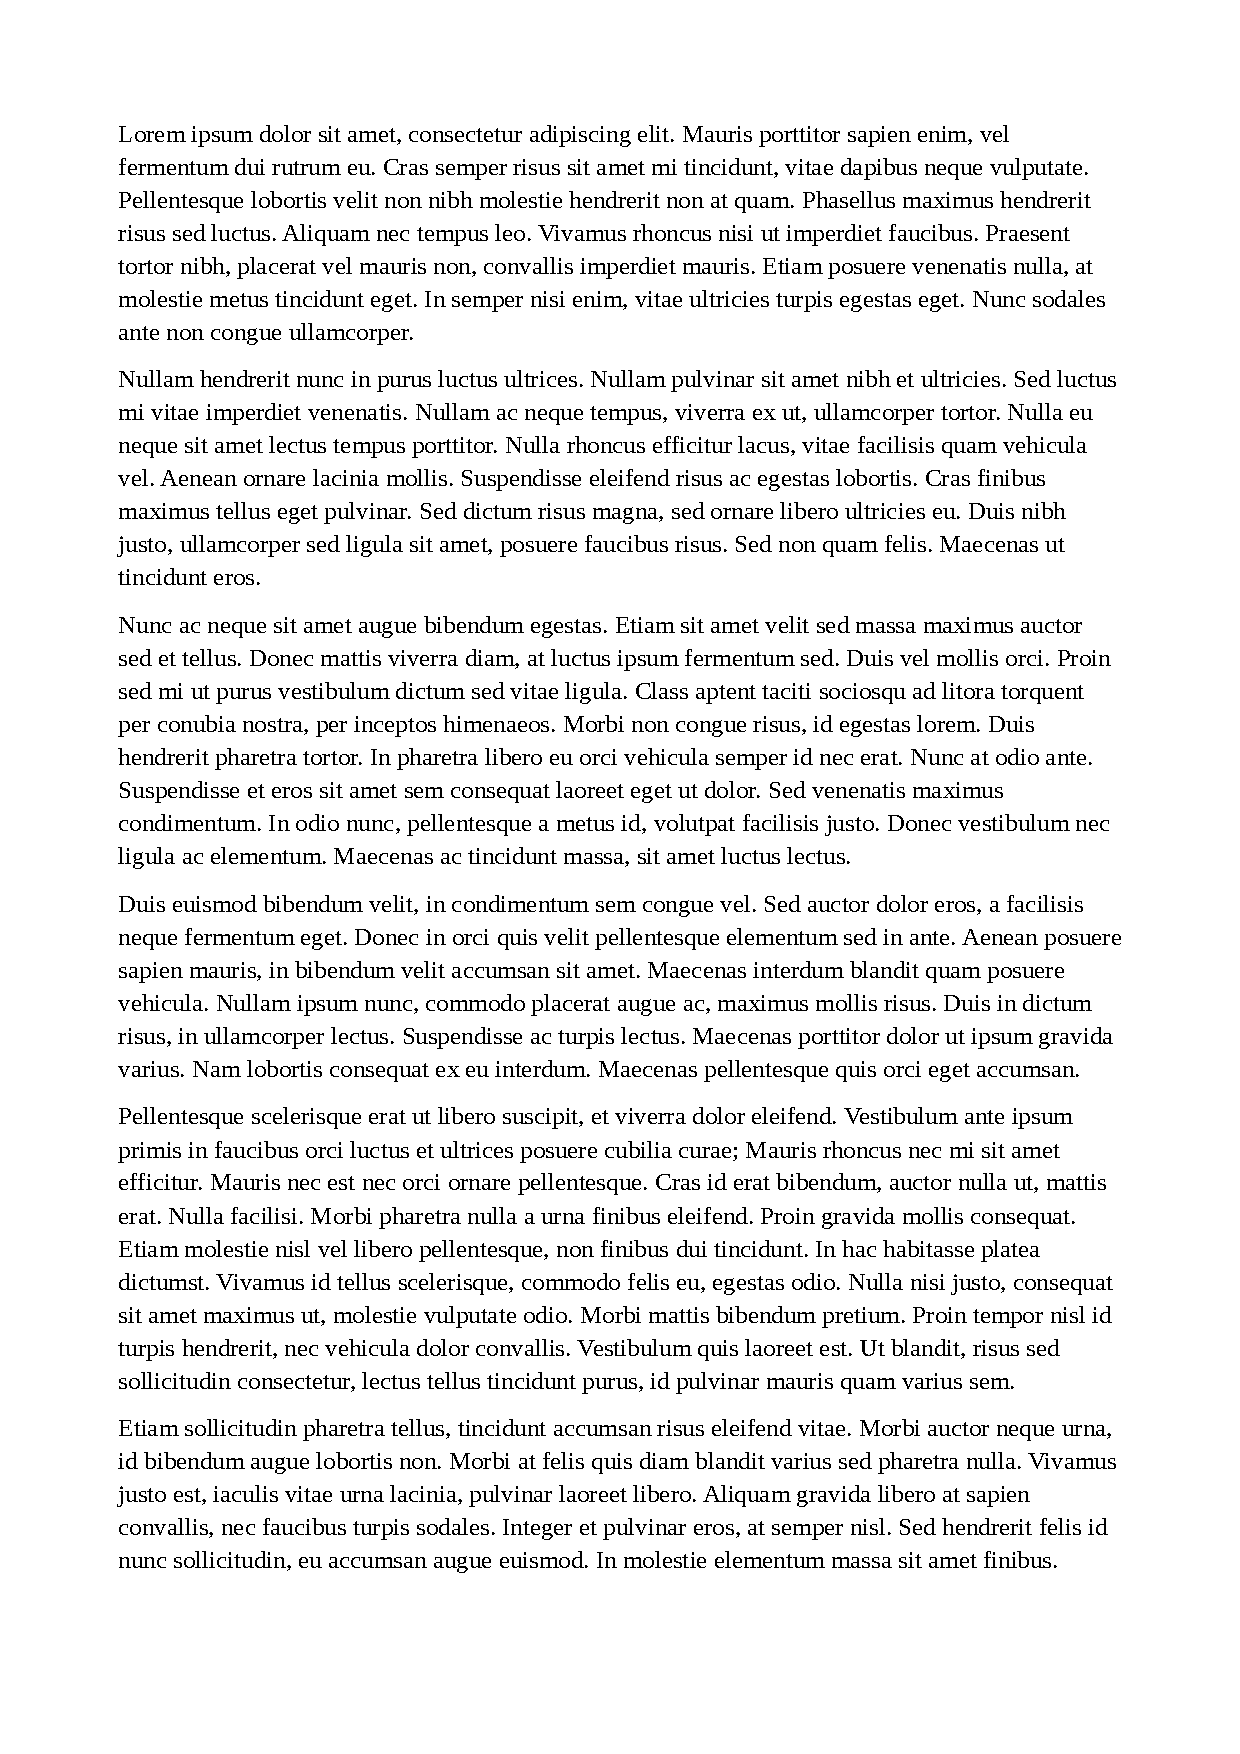
\includepdf[pages={1},scale=0.8,pagecommand=\chapter{Texto Texto Texto Texto}\label{apen:apendiceA}]{appendix/apendiceA}
\includepdf[pages={2-},scale=0.80,pagecommand={}]{appendix/apendiceA}

%%coloca o identificador do anexo/apendice somente na primeira página

\includepdf[pages={1},scale=0.80,pagecommand=\chapter{Texto Texto Texto}\label{apen:apendiceB}]{appendix/apendiceB}


%%coloca o identificador do anexo/apendice somente na primeira página
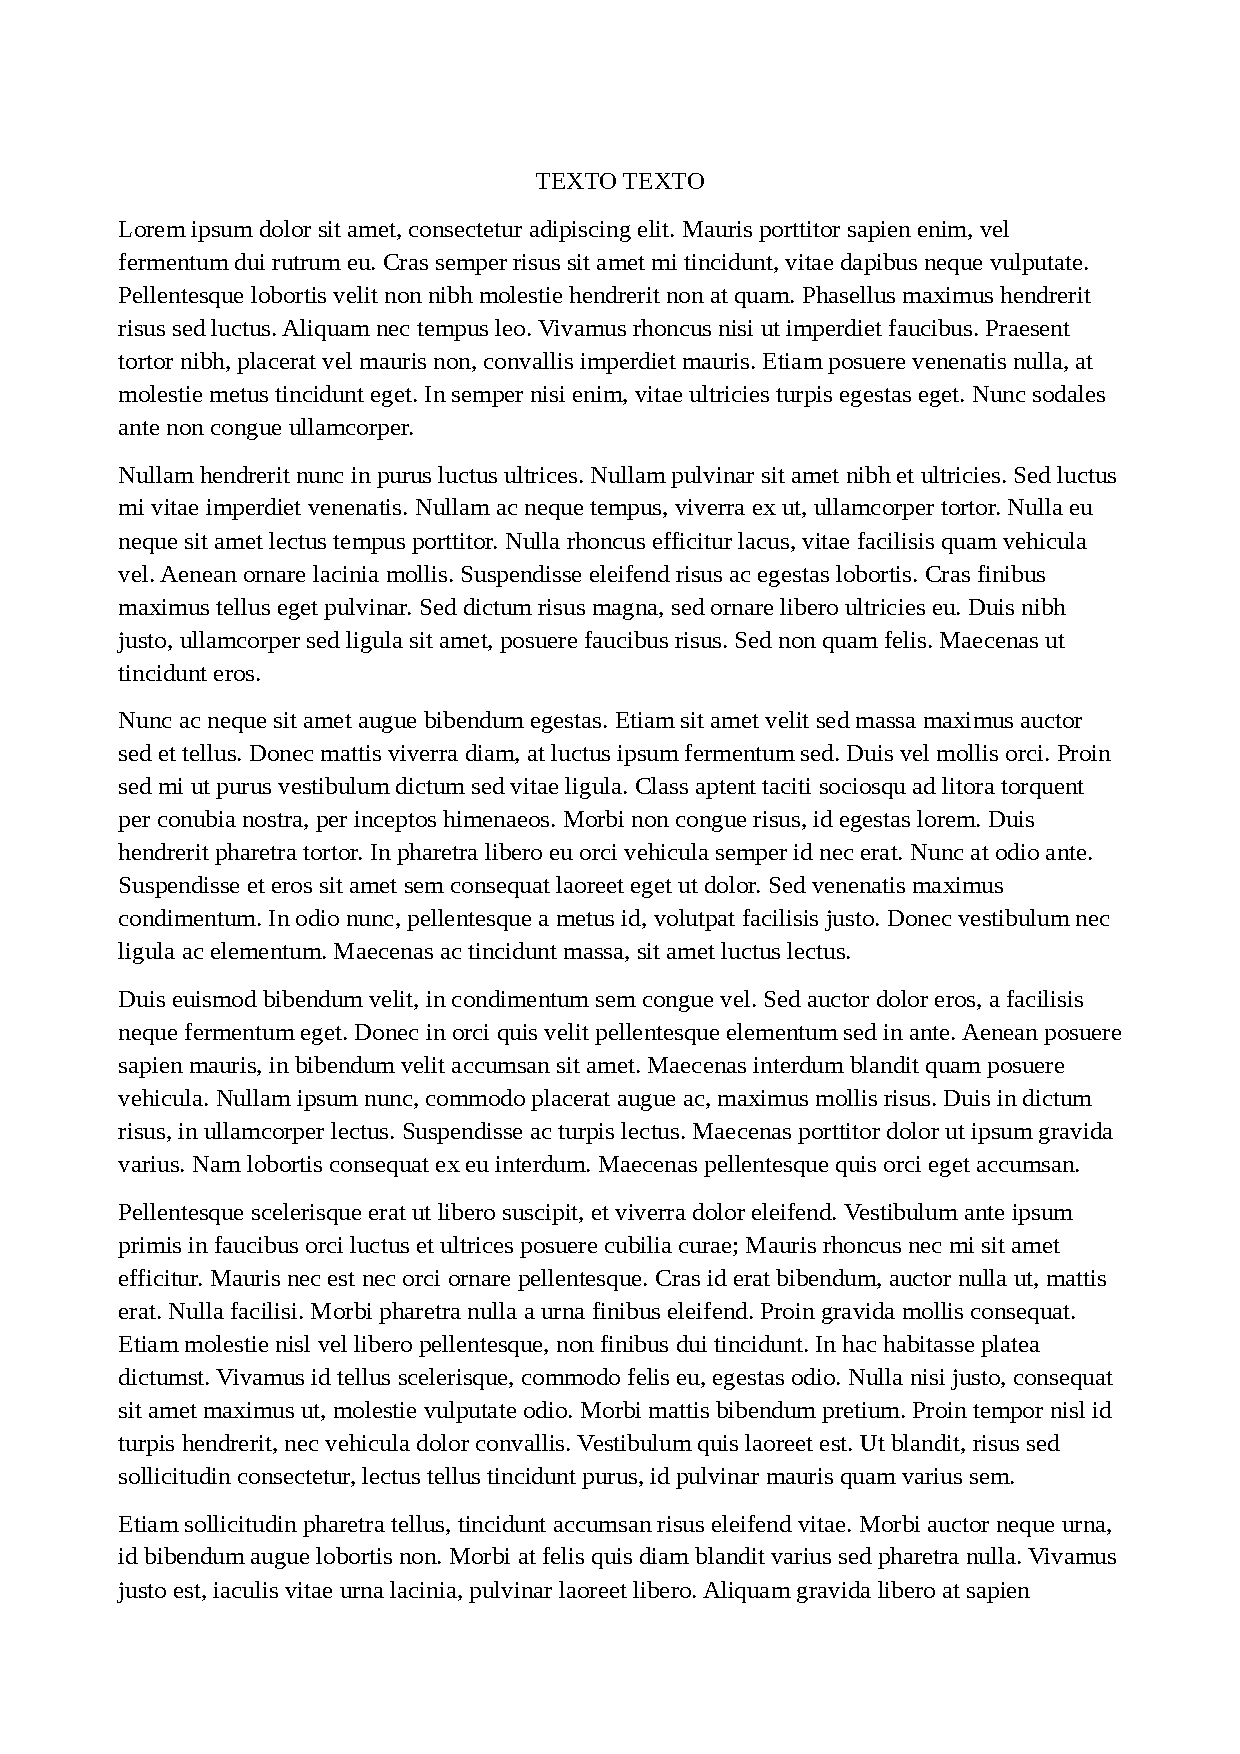
\includepdf[pages={1},scale=0.80,pagecommand=\chapter{Texto Texto}\label{apen:apendiceC}]{appendix/apendiceC}
\includepdf[pages={2},scale=0.80,pagecommand={}]{appendix/apendiceC}




\addtocontents{toc}{\endgroup}
\end{apendicesenv}



% ----------------------------------------------------------
% ANEXOS
% ----------------------------------------------------------
% força para que não exiba subtítulos em apêndices no sumário
\begin{anexosenv}
\addtocontents{toc}{\protect\setcounter{tocdepth}{1}}
\makeatletter
\addtocontents{toc}{%
  \begingroup
  \let\protect\l@chapter\protect\l@section
  \let\protect\l@section\protect\l@subsection
}
\makeatother
% Imprime uma página indicando o início dos apêndices
% \partapendices
% Anexos

%%coloca o identificador do anexo/apendice somente na primeira página
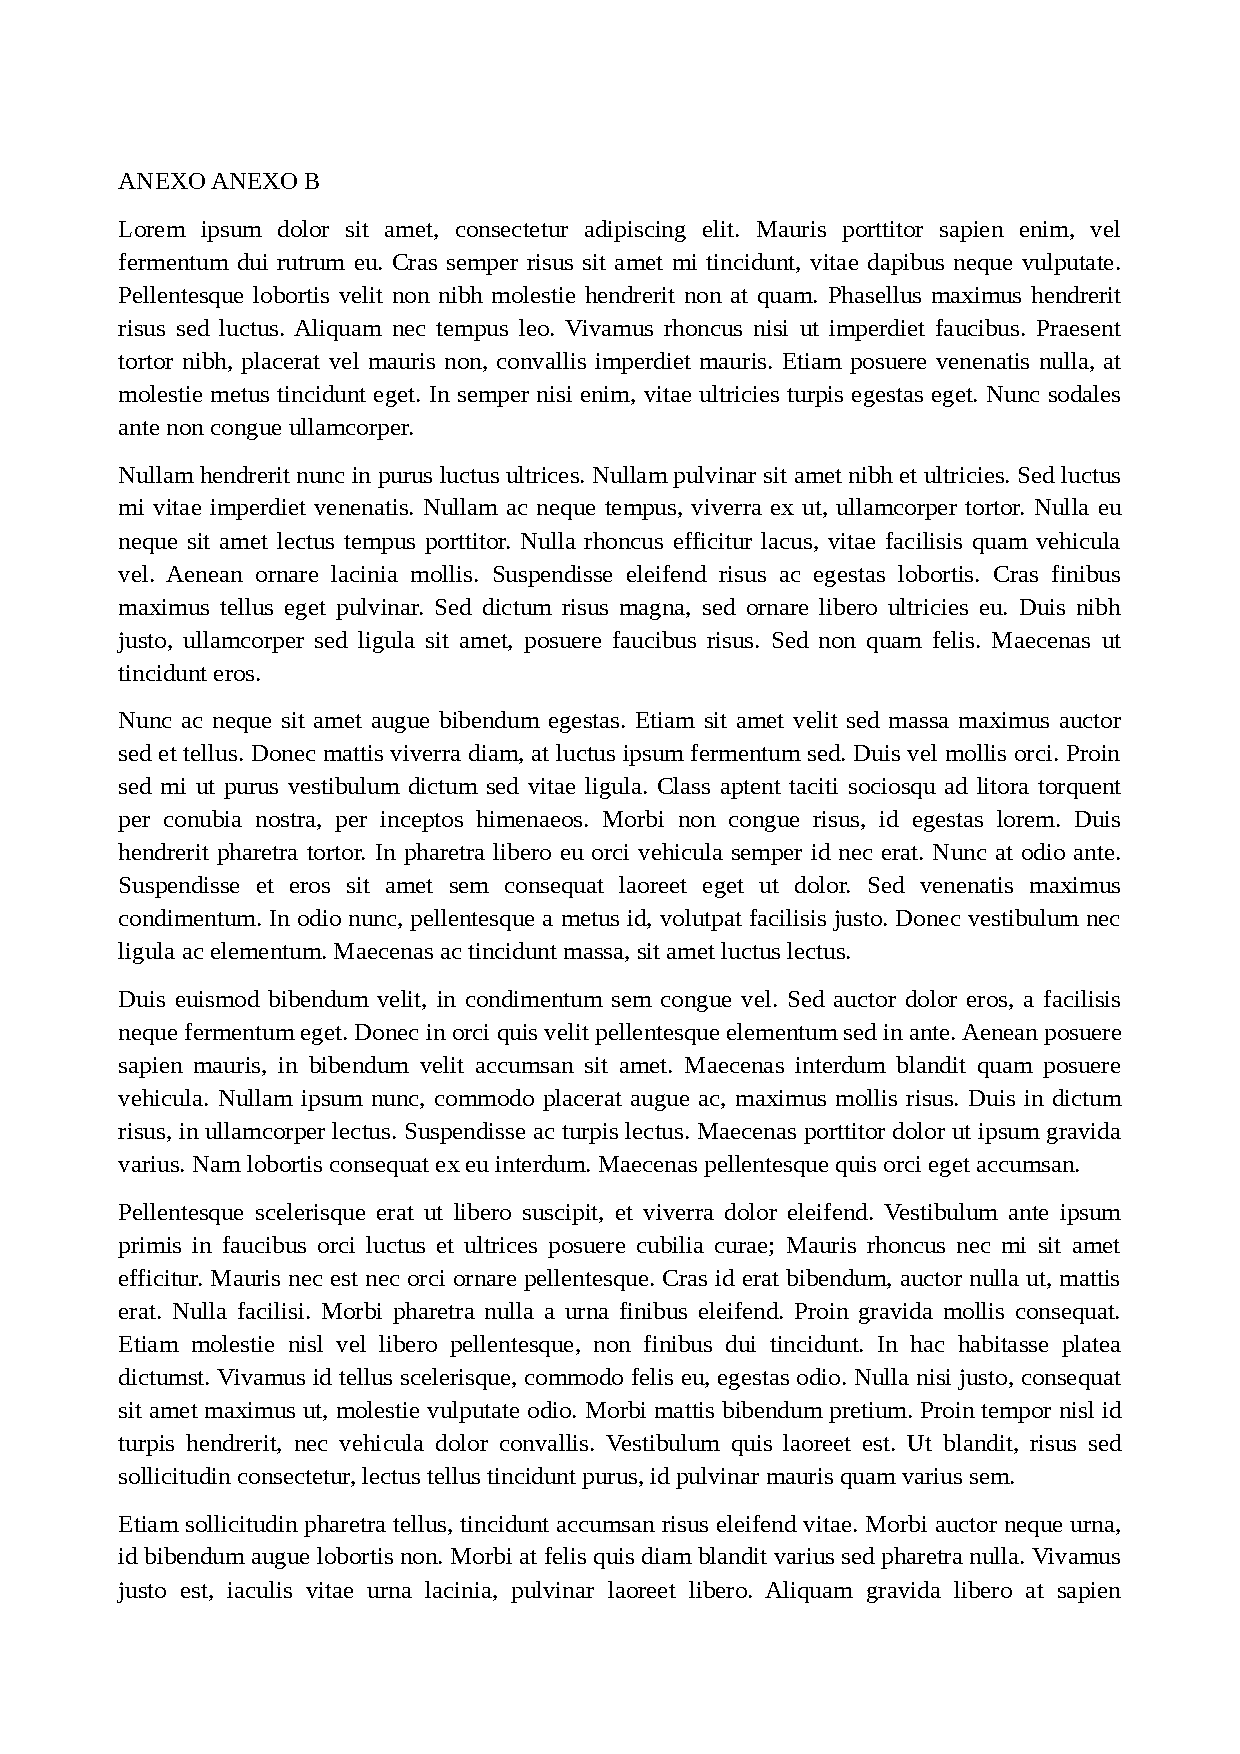
\includepdf[pages={1},scale=0.8,pagecommand=\chapter{Texto Texto Texto Texto}\label{anex:anexob}]{anexos/anexoB}
\includepdf[pages={2-},scale=0.80,pagecommand={}]{anexos/anexoB}

%%coloca o identificador do anexo/apendice somente na primeira página
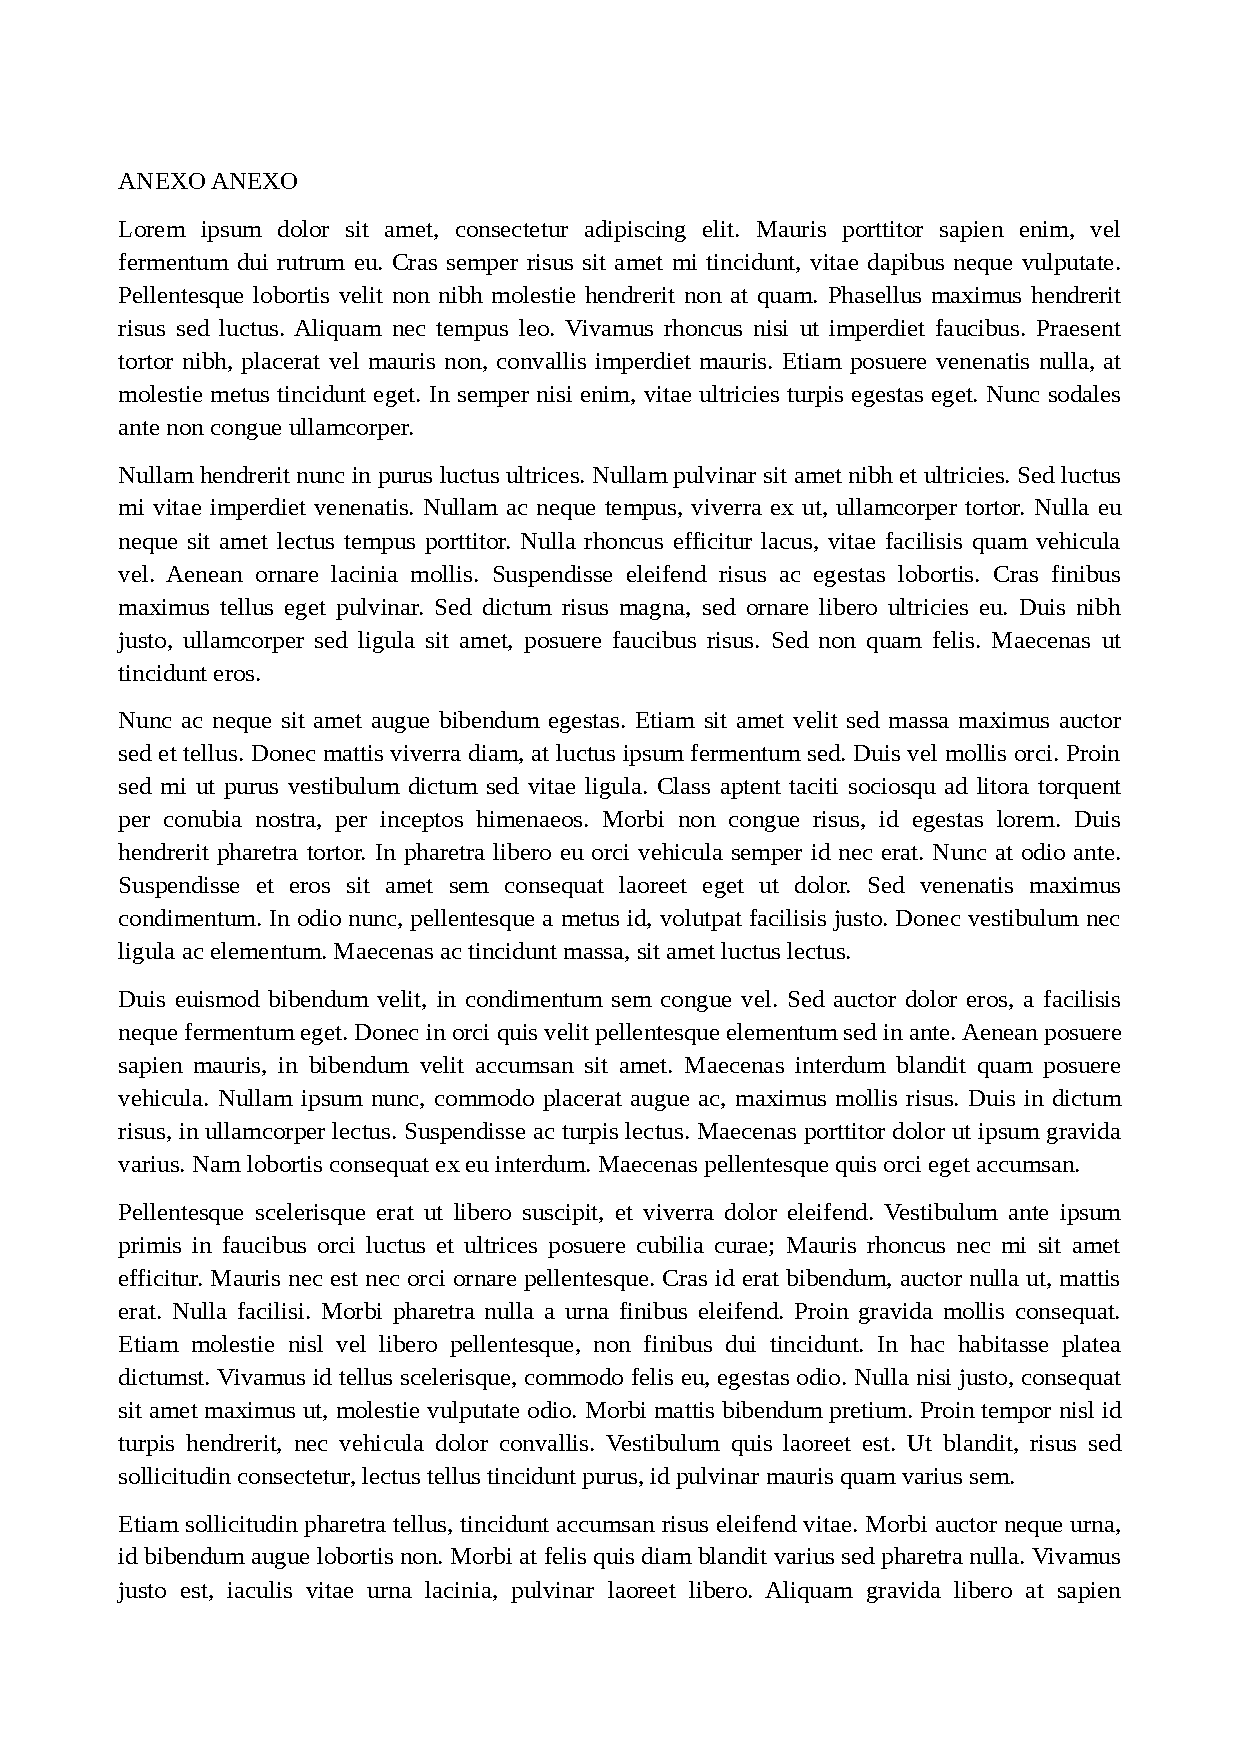
\includepdf[pages={1},scale=0.8,pagecommand=\chapter{Texto Texto Texto Texto}\label{anex:anexoa}]{anexos/anexoA}
\includepdf[pages={2-},scale=0.80,pagecommand={}]{anexos/anexoA}


\addtocontents{toc}{\endgroup}
\end{anexosenv}


% ----------------------------------------------------------
\printindex

\end{document}
